% !TeX program = xelatex
% !TEX root = main.tex
% !TeX encoding = UTF-8
\documentclass[10.5pt,compsoc]{CjC}
%\usepackage{CJKutf8}
%\usepackage{CJK}
\usepackage{graphicx}
\usepackage{footmisc}
\usepackage{subfigure}
\usepackage{url}
\usepackage{multirow}
\usepackage[noadjust]{cite}
\usepackage{amsmath,amsthm}
\usepackage{amssymb,amsfonts}
\usepackage{booktabs}
\usepackage{color}
\usepackage{ccaption}
\usepackage{booktabs}
\usepackage{float}
\usepackage{fancyhdr}
\usepackage{caption}
\usepackage{xcolor,stfloats}
\usepackage{comment}
\setcounter{page}{1}
\graphicspath{{figures/}}
\usepackage{cuted}%flushend,
\usepackage{captionhack}
\usepackage{epstopdf}
% 图片与正文之间的间距
\setlength{\intextsep}{3pt}
% 顶部或底部浮动图片与正文的间距
\setlength{\textfloatsep}{4pt}
% 两个浮动体之间的间距
\setlength{\floatsep}{4pt}

%===============================%
\headevenname{\mbox{\quad} \hfill  \mbox{\zihao{-5}{\songti  计\quad \quad 算\quad \quad 机\quad \quad 学\quad \quad 报 } \hspace {50mm} \mbox{\songti  2026 年 }}}%
\headoddname{\songti  高质量慢病医疗数据的智能标注技术研究}%

%footnote use of *
\renewcommand{\thefootnote}{\fnsymbol{footnote}}
\setcounter{footnote}{0}
\renewcommand\footnotelayout{\zihao{5-}}

\newtheoremstyle{mystyle}{0pt}{0pt}{\normalfont}{1em}{\bf}{}{1em}{}
\theoremstyle{mystyle}
\renewcommand\figurename{figure~}
\renewcommand{\thesubfigure}{(\alph{subfigure})}
\newcommand{\upcite}[1]{\textsuperscript{\cite{#1}}}
\renewcommand{\labelenumi}{(\arabic{enumi})}
\newcommand{\tabincell}[2]{\begin{tabular}{@{}#1@{}}#2\end{tabular}}
\newcommand{\abc}{\color{white}\vrule width 2pt}
\makeatletter
\renewcommand{\@biblabel}[1]{[#1]\hfill}
\makeatother
\setlength\parindent{2em}


\begin{document}
\hyphenpenalty=50000
\makeatletter
\newcommand\mysmall{\@setfontsize\mysmall{7}{9.5}}
\newenvironment{tablehere}
  {\def\@captype{table}}{}

\let\temp\footnote
\renewcommand \footnote[1]{\temp{\zihao{-5}#1}}


\thispagestyle{plain}%
\thispagestyle{empty}%
\pagestyle{CjCheadings}

\begin{table*}[!t]
\vspace {-13mm}
\begin{tabular}{p{168mm}}
\zihao{5-}
\songti 
计\quad 算\quad 机\quad 学\quad 报
\zihao{5-}\songti  
2026年11月 \hfill CHINESE JOURNAL OF COMPUTERS \hfill November. 2026 \\
\hline\\[-4.5mm]
\hline\end{tabular}

\centering
\vspace{11mm}
\heiti  
{\zihao{2} 高质量慢病医疗数据的智能标注技术研究 }

\vskip 5mm

{\zihao{3} \fangsong 
刘存$^{1)}$\quad  杨峥芃$^{1)}$ \quad 巨亚昊$^{1)}$
 }


\vspace{5mm}
\zihao{6}{\songti
$^{1)}$(南开大学 计算机学院，天津市 300350)
}


\vskip 5mm
{\centering
\begin{tabular}{p{160mm}}
\zihao{5-}{
\setlength{\baselineskip}{16pt}\selectfont{
\noindent\heiti 摘\quad 要\quad   \songti  
*中文摘要内容置于此处(英文摘要中要有这些内容)，字体为小5号宋体。摘要贡献部分，要有数据支持，不要出现``...大大提高''、``...显著改善''等描述，正确的描述是``比{\ldots}提高X{\%}''、
``在{\ldots}上改善X{\%}''。*摘要

 \par}}\\[2mm]

\zihao{5-}{\noindent
\heiti 关键词  \quad \songti  {*关键词（中文关键字与英文关键字对应且一致，应有5-7个关键词)；关键词；关键词；关键词*  } }
\end{tabular}}

\vskip 7mm

\begin{center}
\zihao{3}{ {\heiti Research on Intelligent Annotation Technology of High-quality Chronic Disease Medical Data }}\\
\vspace {5mm}
\zihao{5}{ {\heiti Liu Cun$^{1)}$ YangZhengpeng$^{1)}$ JuYahao$^{1)}$ 
}}\\
\vspace {2mm}


\zihao{6}{\heiti {$^{1)}$(Nankai University, School of Computer Science, Tianjin, 300350) } }







\end{center}

\begin{tabular}{p{160mm}}
\zihao{5}{
\setlength{\baselineskip}{18pt}\selectfont{
{\bf Abstract}\quad \begin{heiti} (\textbf{500英文单词，内容包含中文摘要的内容}).
字体为Times new Roman,字号5号* Abstract \end{heiti}
\par}}\\

\setlength{\baselineskip}{18pt}\selectfont{
\zihao{5}{\noindent Do not modify the amount of space before and after the artworks. One- or two-column format artworks are preferred. and Tables, create a new break line and paste the resized artworks where desired. Do not modify the amount of space before and after the artworks. One- or two-column format artworks are preferred. All Schemes, Equations, Figures, and Tables should be mentioned in the text consecutively and numbered with Arabic numerals, and appear below where they are mentioned for the first time in the main text. To insert Schemes, Equations, Figures, and Tables, create a new break line and paste the resized artworks where desired. Do not modify the amount of space before and after the artworks. One- or two-column format artworks are preferred.Do not modify the amount of space before and after the artworks. One- or two-column format artworks are preferred. and Tables, create a new break line and paste the resized artworks where desired. Do not modify the amount of space before and after the artworks. One- or two-column format artworks are preferred. All Schemes, Equations, Figures, and Tables should be mentioned in the text consecutively and numbered with Arabic numerals, and appear below where they are mentioned for the first time in the main text.

\vspace {5mm}
{\bf Keywords}\quad \heiti 中文关键字与英文关键字对应且一致，\textbf{不要用英文缩写});
key word; key word; key word* *字体为5号Times new Roman * Key words }\par}
\end{tabular}



% 已删除收稿日期、基金、作者简介等模板占位信息。
% 保留下面的 \end{table*}：它闭合从封面标题开始的整个浮动环境。
\end{table*}
\clearpage

\linespread{1.15}
\heiti 


\zihao{5}
\vskip 1mm



\section{医学图像智能标注技术研究与实现}
\songti


\subsection{医学影像数据集}

为验证医学图像智能标注方法在不同成像模态和病灶类型下的适用性，本项目选取三套公开医学影像数据集：BUSI、LGG 和 ISIC 2018。三套数据集分别覆盖乳腺超声、脑部磁共振成像和皮肤镜图像，具有不同的成像原理、组织结构和病灶表现形式。与此同时，三套数据集均提供与原始图像对应的像素级分割标注，可作为评价自动分割结果的参考标准。通过在不同医学影像上使用同一预训练模型，可以考察其在跨模态医学图像标注任务中的实际应用能力。

\noindent\textbf{BUSI：乳腺超声图像数据集。}

BUSI（Breast Ultrasound Images）\cite{busi2020}由 Al-Dhabyani 等人整理并公开，相关数据集论文发表于 Data in Brief。该数据集采集自埃及开罗 Baheya 医院，包含来自 600 名女性患者的乳腺超声图像，患者年龄范围为 25--75 岁。原始数据经过筛选和预处理后，共保留 780 张图像，平均图像尺寸约为 $500\times500$ 像素，以 PNG 格式存储。

根据影像对应的临床类别，BUSI 分为正常（Normal）、良性（Benign）和恶性（Malignant）三类，其中正常图像 133 张、良性病变图像 437 张、恶性病变图像 210 张。对于包含乳腺肿块的图像，数据集提供对应的病灶分割 Mask，用于标识病变区域的位置及轮廓。因此，该数据集既可用于乳腺病变分类与检测，也可用于像素级病灶分割研究。

乳腺超声通过组织声学特性的差异形成图像，其成像过程容易受到散斑噪声、组织回声变化和声学伪影的影响。部分乳腺病灶与周围组织之间的灰度对比度较低，且病灶边缘可能存在模糊、不规则等情况，使得精确分割具有一定难度。本项目选用 BUSI，主要用于验证自动标注模型在低对比度超声影像中识别乳腺病灶并生成分割区域的能力。

\begin{figure}[!htbp]
    \centering
    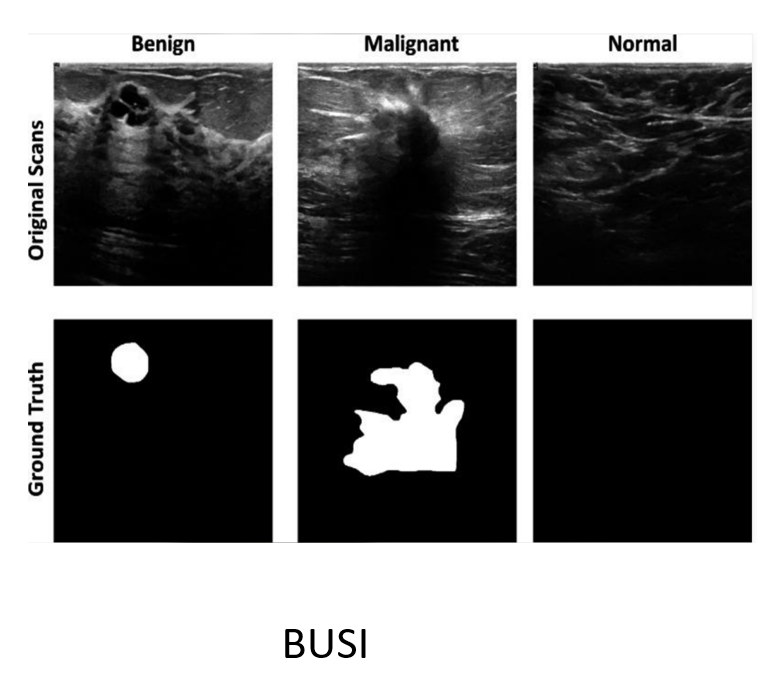
\includegraphics[width=\linewidth,keepaspectratio]{lc-figures/busi.png}
    \caption{\songti BUSI 医学影像及其分割标注示例}
    \label{fig:medical_datasets}
\end{figure}




\noindent\textbf{LGG：低级别胶质瘤脑部 MRI 数据集。}

LGG（Low-Grade Glioma）\cite{lgg2019}数据集主要面向脑部低级别胶质瘤的影像分析与分割任务。其原始医学影像来源于 The Cancer Imaging Archive（TCIA），对应 The Cancer Genome Atlas（TCGA）中的低级别胶质瘤病例。该数据集包含来自 110 名患者的 3929 张二维脑部 MRI 切片，每张图像均配有对应的人工分割 Mask。图像主要采用液体衰减反转恢复（Fluid-Attenuated Inversion Recovery，FLAIR）序列，公开版本中的切片尺寸为 $256\times256$ 像素，以 TIFF 格式存储。数据集中同时包含存在异常信号区域的切片和未显示对应异常区域的切片，因此可用于研究模型对病变区域的识别与分割能力。

FLAIR 是脑部 MRI 中常用的成像序列之一，通过抑制脑脊液信号，使部分脑组织异常区域更容易被观察。该数据集提供的标注主要针对 FLAIR 图像中的异常信号区域，而不是直接反映组织病理学意义上的精确肿瘤边界。

与乳腺超声不同，脑部 MRI 具有较为复杂的解剖结构，病变区域可能分布于不同脑叶，并呈现不同的大小、形状及信号强度。同时，由于原始三维脑部扫描被表示为多个二维切片，相邻切片之间的病灶形态也可能发生明显变化。因此，本项目选择 LGG 数据集，用于验证自动标注模型对脑部复杂解剖背景及不规则异常区域的分割能力。




\begin{figure}[H]
    \centering
    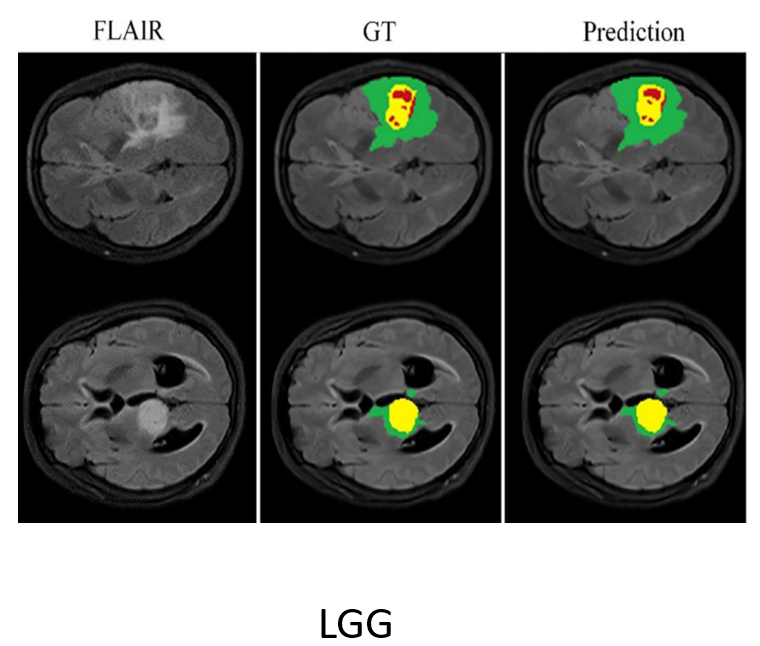
\includegraphics[width=\linewidth,keepaspectratio]{lc-figures/lgg.png}
    \caption{\songti LGG 医学影像及其分割标注示例}
    \label{fig:medical_datasets}
\end{figure}





\noindent\textbf{ISIC 2018：皮肤镜图像数据集。}

ISIC 2018 \cite{isic2018}数据集来源于国际皮肤影像协作组织（International Skin Imaging Collaboration，ISIC）举办的 Skin Lesion Analysis Towards Melanoma Detection 2018 挑战赛。该挑战赛面向皮肤病变分析，设置了病灶边界分割、皮肤镜特征检测和病变诊断等不同任务。

本项目使用其中的 Task 1，即皮肤病灶边界分割（Lesion Boundary Segmentation）任务。该任务共提供 2594 张训练图像、100 张验证图像和 1000 张测试图像，总计 3694 张皮肤镜图像。其中，2594 张训练图像配有对应的专家病灶分割 Mask，能够用于模型训练和分割结果评价。官方验证集和测试集在挑战赛评测阶段主要用于模型性能评估，其标注不作为普通训练数据提供。

与灰度形式的乳腺超声和脑部 MRI 不同，皮肤镜图像通常为彩色图像，可以反映皮肤病灶的颜色、纹理及形态特征。不同病灶之间可能存在显著的颜色与结构差异，而部分病灶与正常皮肤之间的边界并不清晰。此外，毛发遮挡、反光、光照变化和皮肤纹理等因素也可能干扰模型的病灶定位与边界分割。

因此，ISIC 2018 常被用于评价医学图像分割方法在复杂颜色分布、不规则病灶轮廓及局部遮挡条件下的表现。本项目选用该数据集，主要用于验证自动标注模型在彩色皮肤镜图像上的病灶识别与像素级分割能力。



\begin{figure}[H]
    \centering
    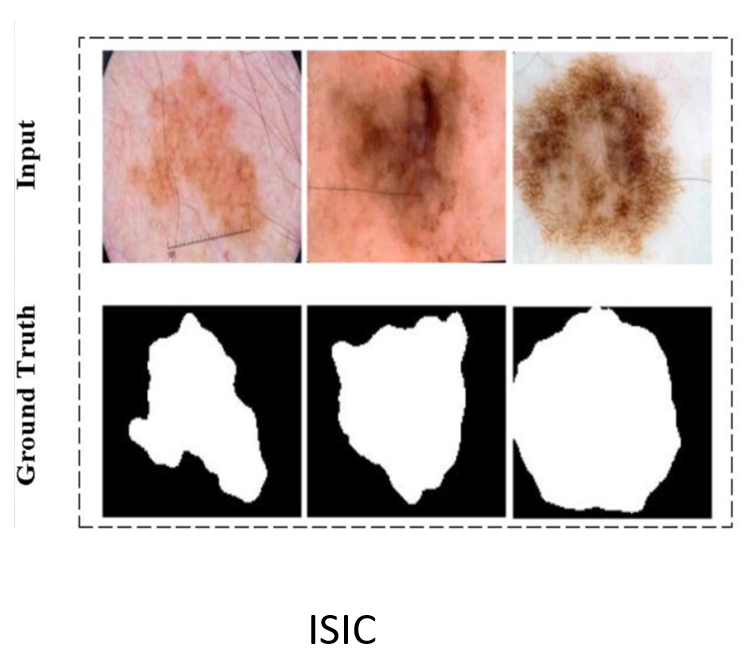
\includegraphics[width=\linewidth,keepaspectratio]{lc-figures/isic.png}
    \caption{\songti ISIC 医学影像及其分割标注示例}
    \label{fig:medical_datasets}
\end{figure}




上述三套数据集分别代表超声、磁共振和皮肤镜三种医学成像方式，在图像通道、组织结构、病灶表现和分割难点方面具有明显差异。因此，相比仅在单一数据集上进行测试，使用多模态医学影像能够更全面地展示智能标注方法的适用范围。





\subsection{评价指标}

为定量评估医学图像智能标注的准确性，本项目采用 Dice 相似系数（Dice Similarity Coefficient，DSC）和交并比（Intersection over Union，IoU）作为主要评价指标。两项指标均广泛应用于医学图像分割任务，通过衡量模型预测区域与人工标注区域之间的重合程度，评价模型对病灶位置及形状的识别能力。

对于每张医学图像，首先将模型预测结果与数据集提供的人工标注转换为相同尺寸的二值分割掩码，其中前景像素表示目标病灶区域，背景像素表示非目标区域。根据预测结果与人工标注之间的对应关系，将像素划分为真正例（True Positive，TP）、假正例（False Positive，FP）、假负例（False Negative，FN）和真负例（True Negative，TN）。其中，TP 表示被正确识别为病灶的像素数量，FP 表示将背景错误识别为病灶的像素数量，FN 表示未被模型识别出的真实病灶像素数量。

\noindent\textbf{Dice 相似系数。}

Dice 系数用于衡量两个分割区域的空间重合程度，是医学图像分割中最常用的评价指标之一。设模型预测的病灶像素集合为 $P$，人工标注的真实病灶像素集合为 $G$，则 Dice 系数定义为：

\begin{equation}
\mathrm{Dice}(P,G)
=
\frac{2|P\cap G|}{|P|+|G|}
=
\frac{2TP}{2TP+FP+FN}.
\label{eq:dice}
\end{equation}

其中，$|P\cap G|$ 表示预测区域与真实区域共同包含的像素数量，$|P|$ 和 $|G|$ 分别表示两个区域的像素数量。Dice 的取值范围为 $[0,1]$，数值越大，说明预测分割结果与人工标注越接近。当 Dice 为 1 时，表示两个区域完全重合；当 Dice 为 0 时，表示两个非空区域不存在重叠。

由于 Dice 系数直接衡量前景区域的重合程度，不受大量正确分类的背景像素影响，因此适用于病灶区域相对较小、前景与背景像素比例不均衡的医学图像分割任务。

\noindent\textbf{（2）交并比。}

IoU 又称 Jaccard 指数，用于衡量预测区域与真实区域的交集占并集的比例，其计算公式如下：

\begin{equation}
\mathrm{IoU}(P,G)
=
\frac{|P\cap G|}{|P\cup G|}
=
\frac{TP}{TP+FP+FN}.
\label{eq:iou}
\end{equation}

其中，$|P\cup G|$ 表示预测区域与真实区域的并集大小。IoU 的取值范围同样为 $[0,1]$，数值越接近 1，表示预测区域与人工标注的一致性越高。

与 Dice 相比，IoU 使用交集与并集的比值衡量分割质量，对错误包含的背景区域以及遗漏的病灶区域均进行惩罚。在相同的预测结果下，IoU 通常不高于 Dice，因此同时报告两项指标能够从不同尺度反映自动分割结果的准确性。

\noindent\textbf{数据集平均评价结果。}

本项目对 BUSI、LGG 和 ISIC 2018 三个数据集分别进行评价。对于每个数据集，首先计算单张测试图像的 Dice 和 IoU，再对全部测试样本的指标取算术平均，得到该数据集上的平均分割性能：

\begin{equation}
\overline{\mathrm{Dice}}
=
\frac{1}{N}
\sum_{i=1}^{N}\mathrm{Dice}_i,
\qquad
\overline{\mathrm{IoU}}
=
\frac{1}{N}
\sum_{i=1}^{N}\mathrm{IoU}_i.
\label{eq:mean_metrics}
\end{equation}

其中，$N$ 为测试图像数量，$\mathrm{Dice}_i$ 和 $\mathrm{IoU}_i$ 分别表示第 $i$ 张图像的评价结果。











\subsection{代表性方法调研}

医学图像分割是计算机视觉技术在医学影像分析中的重要应用，其目标是对图像中的器官、组织或病灶进行像素级识别，获得目标区域的位置、形状及边界信息。传统医学图像分割方法通常依赖针对特定数据集训练的监督学习模型，例如 U-Net 及其改进网络。这类方法能够在训练数据分布相对稳定的情况下取得较好的分割效果，但当医学影像模态、目标器官或病灶类型发生变化时，通常需要重新收集标注数据并训练或微调模型。

随着视觉基础模型的发展，研究人员开始探索利用统一模型处理多种医学图像分割任务。与传统的任务专用模型不同，此类方法通过预训练获得跨任务的视觉表示，并借助不同形式的提示信息指定分割目标，使模型能够在无需额外训练或仅需少量人工交互的情况下完成新任务。

从目标指定方式来看，现有代表性方法可以划分为四类：第一类是基于少样本示例的分割方法，通过已标注的参考图像定义目标；第二类是基于空间位置提示的方法，通过点或边界框指定待分割区域；第三类是基于通用视觉概念的方法，利用自然语言或视觉示例识别目标；第四类是面向医学领域的文本语义分割方法，利用医学术语直接指定目标器官或病灶。

本节选取 UniverSeg、MedSAM、SAM 3 和 BiomedParse 四项代表性工作进行分析，重点比较其任务定义、模型结构、输入提示形式、实验结果及实际应用限制，为后续医学图像智能标注系统的技术选型提供依据。

\subsubsection{UniverSeg：少样本医学图像分割}

UniverSeg 是 Butoi 等人在 ICCV 2023 上提出的通用医学图像分割方法\cite{universeg2023}。该方法主要针对传统医学分割模型跨任务泛化能力不足的问题，探索如何在不重新训练模型的情况下，直接完成新的医学图像分割任务。

\noindent\textbf{研究背景与核心问题。}

医学图像分割任务具有较强的异质性。一方面，不同成像设备产生的数据存在显著差异，例如 CT 和 MRI 主要反映人体内部组织结构，而超声图像具有明显的散斑噪声和回声特征；另一方面，即使使用相同的医学图像，不同应用也可能要求分割完全不同的目标。例如，对于一张腹部 CT 图像，研究人员可能希望分割肝脏、肾脏或某一特定病灶。

传统监督学习模型通常针对预先确定的分割任务进行训练。当分割目标发生变化时，需要重新提供目标类别对应的人工标注，并对模型参数进行更新。这不仅增加了计算资源消耗，也提高了医疗研究人员使用深度学习分割工具的技术门槛。

针对上述问题，UniverSeg 提出一种无需针对新任务微调的医学图像分割框架。其核心思想是：不再将分割任务完全编码在模型参数中，而是在推理阶段通过少量已经标注的参考图像，动态告诉模型当前需要完成什么分割任务。

\noindent\textbf{Query--Support 分割框架。}

UniverSeg 将输入划分为查询图像（Query Image）和支持集（Support Set）两部分。Query 表示需要进行自动分割的新图像，Support Set 则由若干组已经标注的医学图像及其分割掩码组成。


\begin{figure*}[!t]
    \centering
    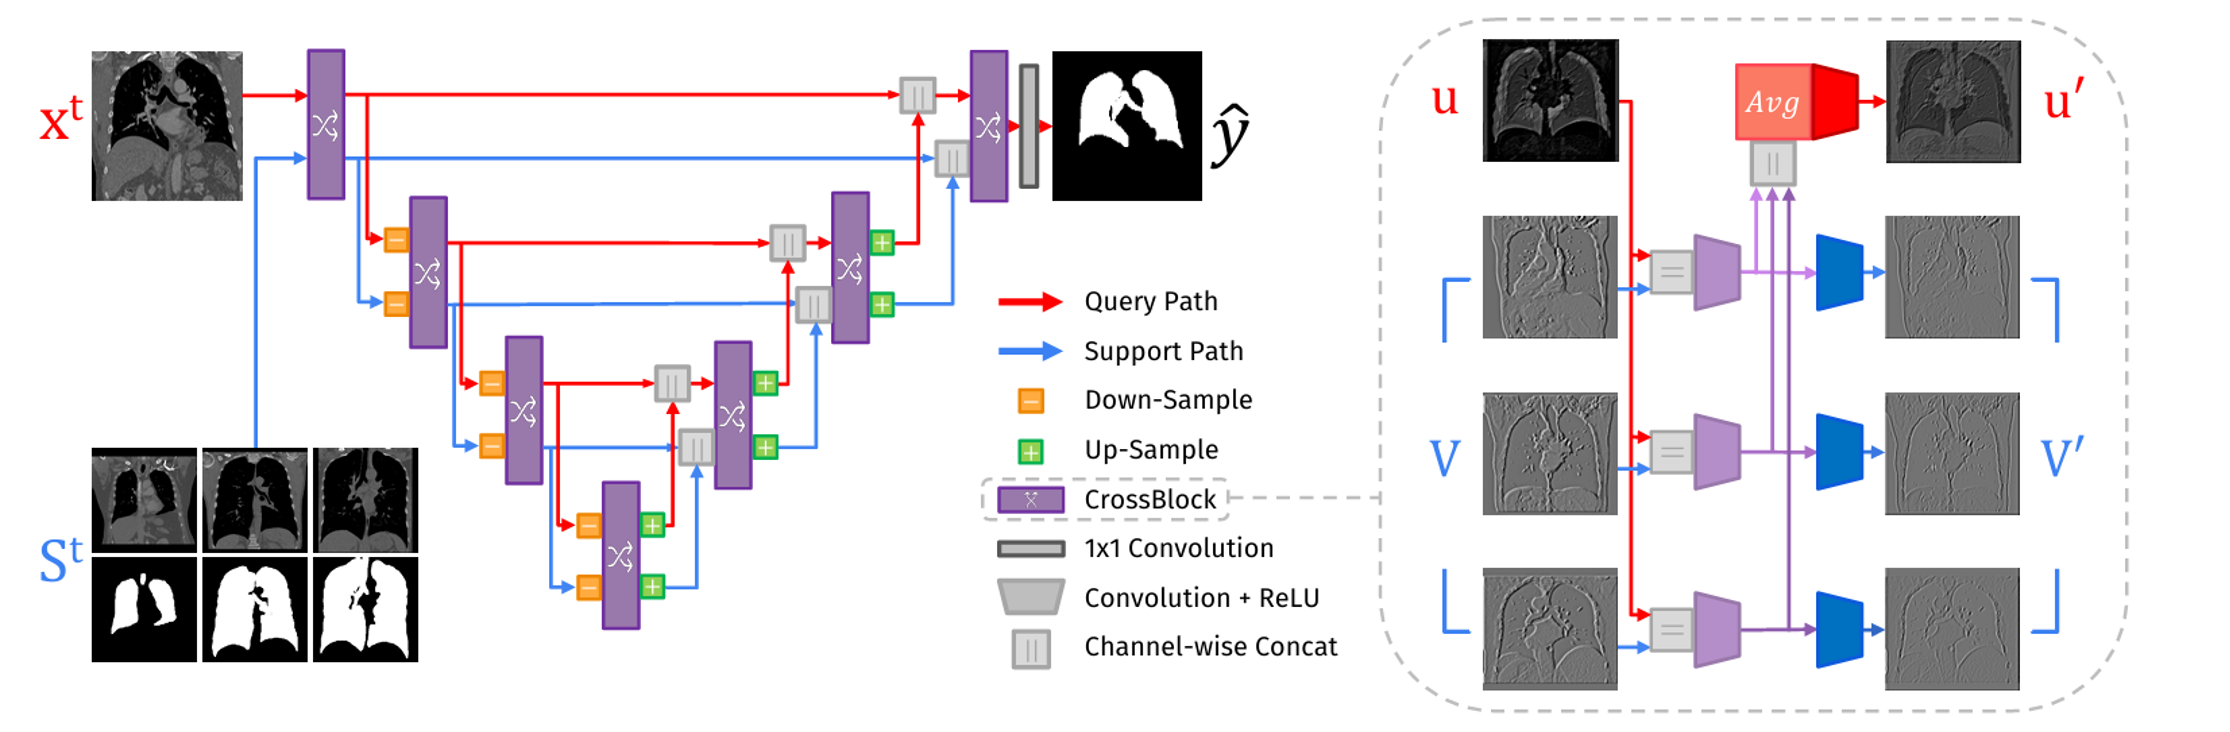
\includegraphics[width=0.7\textwidth,keepaspectratio]{lc-figures/univer.png}
    \caption{\songti UniverSeg 方法示例}
    \label{fig:universeg}
\end{figure*}




设查询图像为 $x_q$，支持集定义为：

\begin{equation}
S=\{(x_i,y_i)\}_{i=1}^{K},
\label{eq:universeg_support}
\end{equation}

其中，$x_i$ 表示第 $i$ 张参考图像，$y_i$ 为其对应的人工分割 Mask，$K$ 为参考样本数量。

UniverSeg 学习一个统一的分割函数：

\begin{equation}
\hat{y}_q=f_{\theta}(x_q,S),
\label{eq:universeg_forward}
\end{equation}

其中，$\theta$ 表示预训练模型的固定参数，$\hat{y}_q$ 表示查询图像的预测分割结果。

与传统模型 $\hat{y}=f_{\theta}^{t}(x)$ 不同，UniverSeg 不需要为每一个任务 $t$ 单独训练模型，而是通过输入支持集 $S$ 表达任务信息。模型根据参考图像与对应 Mask 的关系，推断需要在查询图像中识别和分割的目标。

例如，当需要分割脑部 MRI 中的特定组织时，可以向模型提供数张已经完成该组织分割的 MRI 图像及其 Mask。模型通过分析这些参考样例中的视觉特征与标注区域之间的对应关系，在新的 MRI 图像中预测同类组织的位置。

\noindent\textbf{CrossBlock 特征交互机制。}

UniverSeg 的核心模块是 CrossBlock，其主要作用是实现查询图像特征与参考样本特征之间的信息交互。

模型整体采用类似 U-Net 的编码器--解码器结构，但与传统 U-Net 仅对单张图像提取特征不同，UniverSeg 在不同网络层级中同时处理 Query 特征和 Support 特征。

在 CrossBlock 中，模型首先将查询图像的特征与每个参考样本的特征沿通道维度拼接，然后通过共享参数的卷积操作提取联合表示。对于查询特征 $\mathbf{u}$ 和第 $i$ 个参考特征 $\mathbf{v}_i$，可以表示为：

\begin{equation}
\mathbf{z}_i=
\phi\left(
\operatorname{Conv}
([\mathbf{u};\mathbf{v}_i])
\right),
\label{eq:universeg_cross}
\end{equation}

其中，$[\cdot;\cdot]$ 表示通道拼接，$\operatorname{Conv}$ 表示卷积操作，$\phi$ 表示非线性激活函数。

随后，模型对多个参考样本产生的联合特征进行聚合，并据此更新查询图像的特征表示。与此同时，各参考样本的特征也得到相应更新，从而在多个网络层级中不断交换信息。

这种机制使模型可以综合利用多个参考样本的信息，而不是仅依赖单张示例。其编码器通过逐级下采样提取多尺度语义特征，解码器再通过上采样和跨层特征连接恢复空间分辨率，最终输出像素级预测 Mask。

\noindent\textbf{训练策略与实验结果。}

为了使模型适应不同医学图像任务，作者构建了 MegaMedical 数据集合，整合了 53 套公开医学分割数据集，包含超过 22000 个医学扫描样本，覆盖多种成像模态、解剖部位和分割目标。

在训练过程中，模型反复从不同任务中采样查询图像及参考样本，并利用人工分割标签进行监督学习。作者还引入任务级数据增强，通过改变图像和标注的组织形式，提高模型对未知任务的适应能力。

在实验中，作者采用未参与训练的医学分割任务评价模型泛化能力。结果表明，UniverSeg 在论文所设置的留出任务上取得了约 71.8 的平均 Dice 得分，明显超过所比较的 PANet、ALPNet 和 SENet 等少样本分割方法。

实验还表明，支持样本的数量和多样性会影响模型性能。随着参考样本数量增加，模型通常能够获得更充分的任务信息；当不同参考集合产生的预测结果进行集成时，模型的分割稳定性也可以得到改善。

\noindent\textbf{方法优势与局限。}

UniverSeg 的主要优势是将任务定义从固定模型参数转移到推理阶段的参考样本中，使一个预训练模型能够处理多种新的医学图像分割任务，而无需为每个任务重新训练。

对于已经积累少量人工标注数据的医疗研究团队，这种方式能够降低新任务的模型部署成本，并提高已有标注数据的利用效率。

然而，UniverSeg 并未完全消除人工标注需求。在处理新任务时，系统仍需预先准备具有代表性的图像与 Mask。对于尚未建立标注样本库的医学场景，这一前置条件仍然会产生一定的人工成本。

此外，模型性能与支持集的选择密切相关。当参考样本与待分割图像之间存在明显差异，或者参考样本无法充分表达目标的形态变化时，预测结果可能受到影响。因此，UniverSeg 更适合已有少量可靠标注样本的新任务适配场景，而不是完全依靠目标名称生成预标注的应用场景。

\subsubsection{MedSAM：位置提示驱动的医学图像分割}

MedSAM 是 Ma 等人在 Nature Communications 2024 上提出的医学图像分割基础模型\cite{medsam2024}。该研究针对通用分割模型 Segment Anything Model（SAM）在医学影像中直接应用时存在的性能不足，通过大规模医学影像训练实现领域适配。

\noindent\textbf{研究背景与技术动机。}

SAM 在自然图像分割任务中表现出较强的泛化能力，其主要思想是通过点、边界框或其他形式的提示信息指定目标，再由统一的分割网络生成对应 Mask。

然而，医学图像与自然图像在视觉特征上存在明显差异。自然图像中的物体通常具有较为清晰的外观和边界，而医学影像中的目标可能表现为低对比度区域、复杂内部纹理或形态不规则的异常组织。

例如，在乳腺超声图像中，肿块与周围组织的回声差异可能较小；在脑部 MRI 中，不同组织之间的信号强度存在变化，异常区域的轮廓也可能难以准确识别。

因此，虽然通用 SAM 能够利用空间提示指定目标，但其自然图像预训练特征并不一定能够充分表达医学影像中的细粒度结构。

MedSAM 的研究目标是保留 SAM 提示驱动分割的基本框架，同时利用大规模医学数据提升模型对不同医学影像的适应能力。

\noindent\textbf{模型结构与分割流程。}

MedSAM 沿用 SAM 的三个核心组件：图像编码器（Image Encoder）、提示编码器（Prompt Encoder）和分割解码器（Mask Decoder）。

首先，输入医学图像经过视觉 Transformer 编码器，转换为高维图像特征表示。作者选择 ViT-Base 作为视觉主干网络，在计算效率与特征表达能力之间取得平衡。

在原论文的标准设置中，输入图像被调整为 $1024\times1024$ 分辨率，经过图像编码器后得到 $64\times64$ 的空间特征表示。

其次，用户通过边界框指定需要分割的器官或病灶区域。提示编码器将边界框的左上角和右下角坐标转换为位置相关的特征表示，从而向模型提供目标的空间约束信息。

最后，Mask Decoder 将图像特征与提示特征进行融合，利用注意力机制建立两者之间的关联，输出目标区域的像素级分割概率，并恢复到与原始图像对应的空间分辨率。



\begin{figure*}[!t]
    \centering
    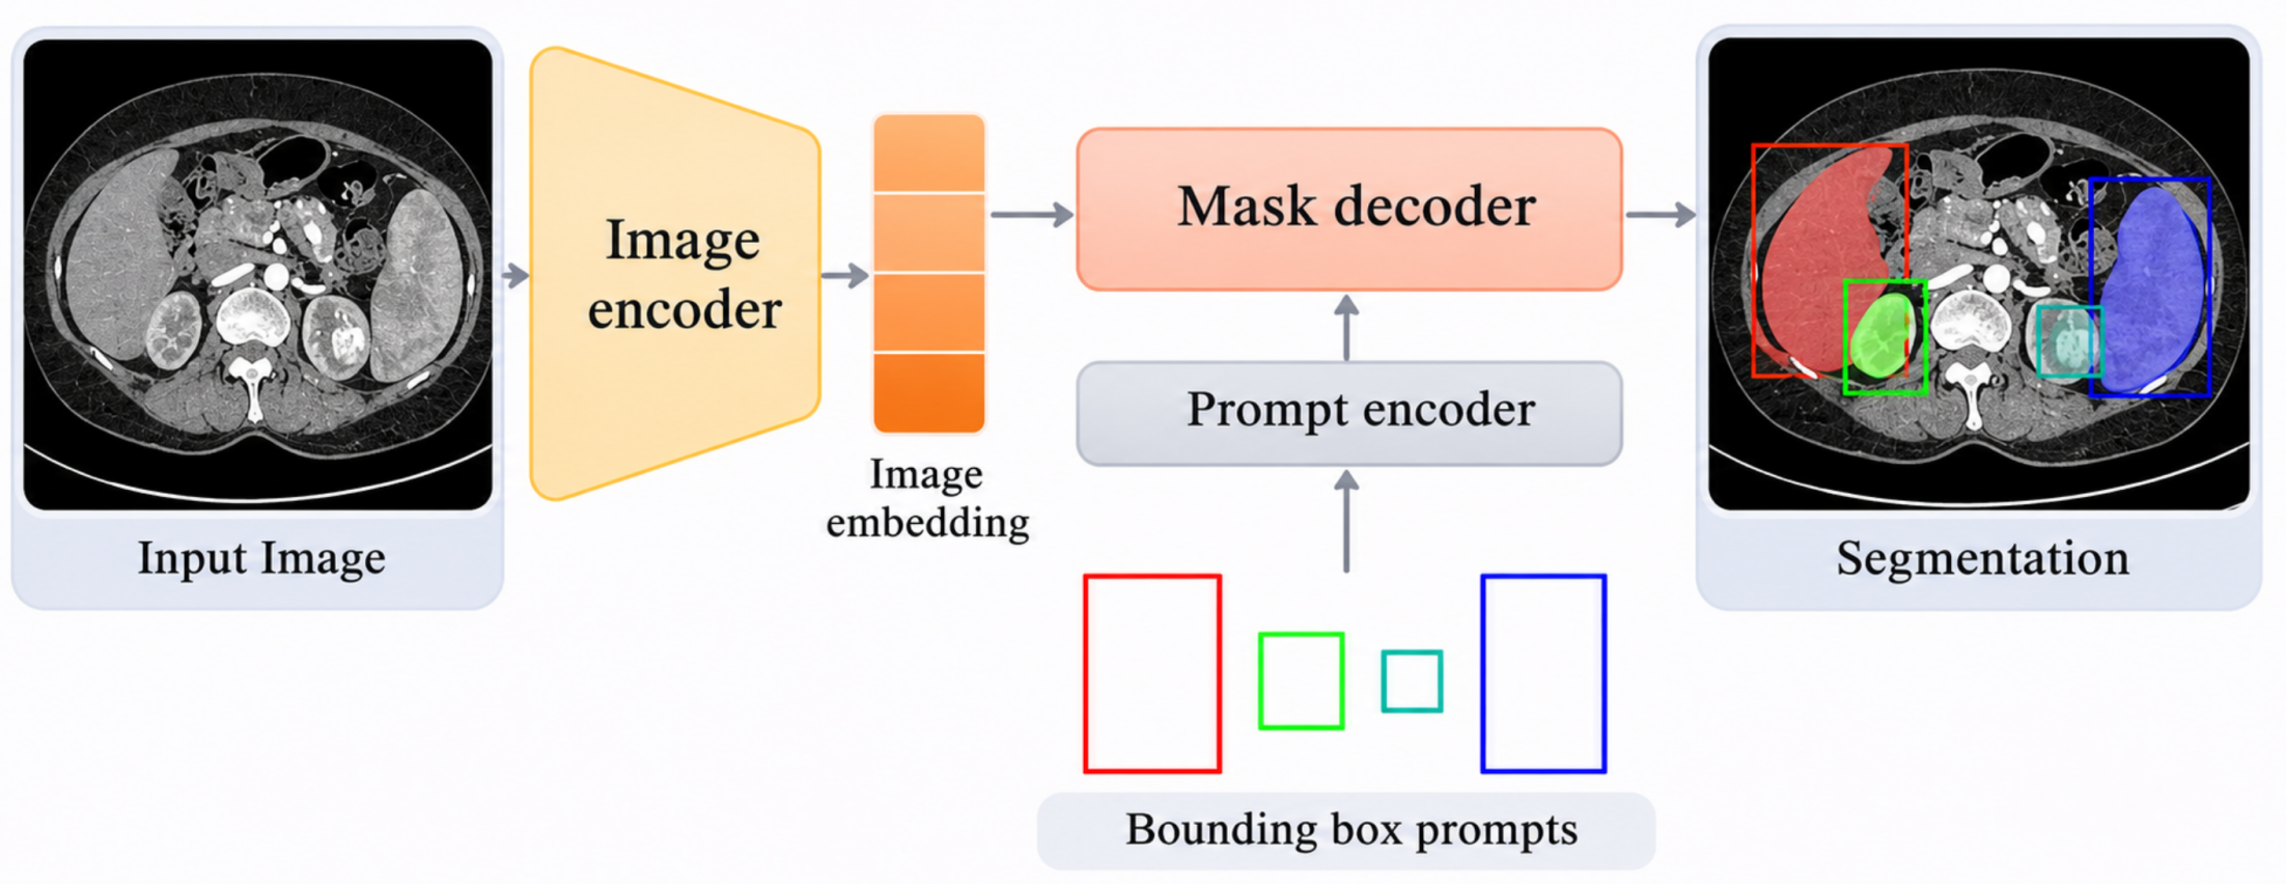
\includegraphics[width=0.7\textwidth,keepaspectratio]{lc-figures/medsam.png}
    \caption{\songti MedSAM 方法示例}
    \label{fig:medsam}
\end{figure*}





对于同一幅医学图像，如果输入不同的边界框，模型可以生成不同目标的分割结果。例如，在腹部 CT 图像中，用户可以分别框选肝脏、脾脏或肾脏，模型根据不同位置提示生成对应的分割 Mask。

这种方式保留了交互式分割的灵活性，并使模型能够在不同医学任务之间复用。

\noindent\textbf{医学领域预训练与优化策略。}

为了提高模型在医学领域中的泛化能力，作者汇总并整理了大规模医学图像分割数据，最终获得 1570263 组图像与分割 Mask，覆盖 10 种医学成像模态及 30 多种癌症类型。

数据集包含 CT、MRI、超声、皮肤镜、内窥镜、病理图像等多种类型，因此能够为模型提供丰富的医学结构和病灶形态信息。

在训练阶段，MedSAM 使用已有的 SAM 预训练权重进行初始化。由于原有提示编码器已经能够表示边界框坐标，因此作者冻结提示编码器参数，主要更新图像编码器和 Mask 解码器，以增强模型的医学影像特征提取能力和分割能力。

训练时，模型根据人工标注的真实 Mask 生成目标边界框，并对边界框坐标施加一定范围的随机扰动，模拟实际使用中用户框选目标时可能产生的位置误差。

优化目标结合 Dice Loss 和交叉熵损失，使模型同时关注预测区域与真实区域的重合程度以及像素级分类准确性。

与简单地在某一种医学数据集上微调 SAM 不同，MedSAM 通过整合大规模跨模态数据，希望获得能够适用于多种器官和病灶类型的通用医学视觉表示。

\noindent\textbf{实验设置与主要结果。}

MedSAM 的原论文设计了较大规模的性能验证，涉及 86 项内部验证任务和 60 项外部验证任务。

其中，内部验证主要考察模型在所构建数据体系中的分割性能；外部验证则使用未参与模型训练的数据集，重点分析模型在不同患者、不同采集条件及新任务中的适用性。

作者将 MedSAM 与原始 SAM，以及针对特定医学影像模态训练的 U-Net、DeepLabV3+ 等模型进行比较。实验结果表明，经过医学领域适配后，MedSAM 在多种医学分割任务中取得了优于原始 SAM 的结果，并在部分任务中达到或超过专用分割模型的性能。

值得注意的是，MedSAM 的优势不仅体现在分割准确率上，还体现在跨任务复用方面。对于不同的医学影像模态，研究人员可以使用相同的预训练模型，只需改变输入图像和目标提示，而不需要维护多个完全独立的分割网络。

\noindent\textbf{方法优势与局限。}

MedSAM 证明了通过大规模医学领域数据适配通用视觉基础模型，可以显著提高模型在医学图像中的实用性。其分割框架相对统一，能够覆盖多种成像模态，也适合与人工交互式标注工具结合使用。

但 MedSAM 的核心工作流程仍然需要位置提示，尤其是目标边界框。用户通常必须事先判断待分割目标位于图像中的什么位置，再通过框选向模型提供空间信息。

如果希望直接对大量尚未标注的医学图像进行自动预标注，那么还需要人工逐张框选目标，或者额外引入目标检测模型生成边界框。

前者会增加人工操作成本，后者则会将目标定位误差传递给后续的分割模型。

此外，对于血管等细长、分支复杂的解剖结构，矩形边界框可能无法明确区分相邻或重叠的目标结构。因此，边界框提示在提供清晰空间约束的同时，也存在目标语义表达不足的问题。

总体而言，MedSAM 更适合目标位置已知或可以方便获得位置提示的医学图像交互式分割场景。对于希望直接通过医学术语生成病灶 Mask 的自动预标注任务，其应用流程仍然存在一定限制。

\subsubsection{SAM 3：通用概念提示分割}

SAM 3 是 Carion 等人提出的通用视觉分割基础模型，相关工作发表于 ICLR 2026\cite{sam32026}。与早期主要依靠点、框等空间提示的分割模型相比，SAM 3 将目标指定方式进一步扩展到开放词汇概念提示，实现图像和视频中的目标检测、分割与跟踪。

\noindent\textbf{研究问题与任务定义。}

传统提示分割模型通常要求用户指出目标的具体位置，例如点击图像中的某个对象，或者使用边界框选定感兴趣区域。

这种交互方式虽然能够生成准确的局部分割结果，但当图像包含大量同类对象时，用户往往需要重复指定目标，难以实现基于语义类别的批量分割。

例如，如果需要分割一张图像中的所有企鹅，传统空间提示方法可能要求用户逐个指定目标，而基于文本概念的分割方法则可以直接输入 a penguin，由模型寻找并分割所有符合该概念的对象。

为此，SAM 3 提出可提示概念分割（Promptable Concept Segmentation，PCS）任务。该任务允许用户通过简短的名词短语、参考图像或者二者的组合指定目标概念，由模型返回图像或视频中所有匹配对象的实例分割结果。

与传统单目标交互式分割不同，PCS 不仅要求模型准确描绘已知目标的轮廓，还要求模型根据语义信息判断图像中是否存在指定对象，以及哪些对象符合输入概念。

\noindent\textbf{检测与跟踪解耦的模型架构。}

SAM 3 采用检测器（Detector）与跟踪器（Tracker）相结合的结构。两个模块共享视觉主干网络，但分别负责当前图像中的目标发现与视频时序中的目标传播。

对于输入的文本概念，模型首先通过文本编码器提取语义特征，并与图像编码器得到的视觉特征进行交互。

随后，基于 DETR 思路构建的检测分支根据语义条件预测候选目标，并为符合要求的对象生成分割 Mask。

为了提高模型区分相近概念的能力，SAM 3 进一步引入目标存在性预测分支（Presence Head），将目标是否存在的语义判断与目标空间位置预测进行一定程度的解耦。

\begin{figure*}[!t]
    \centering
    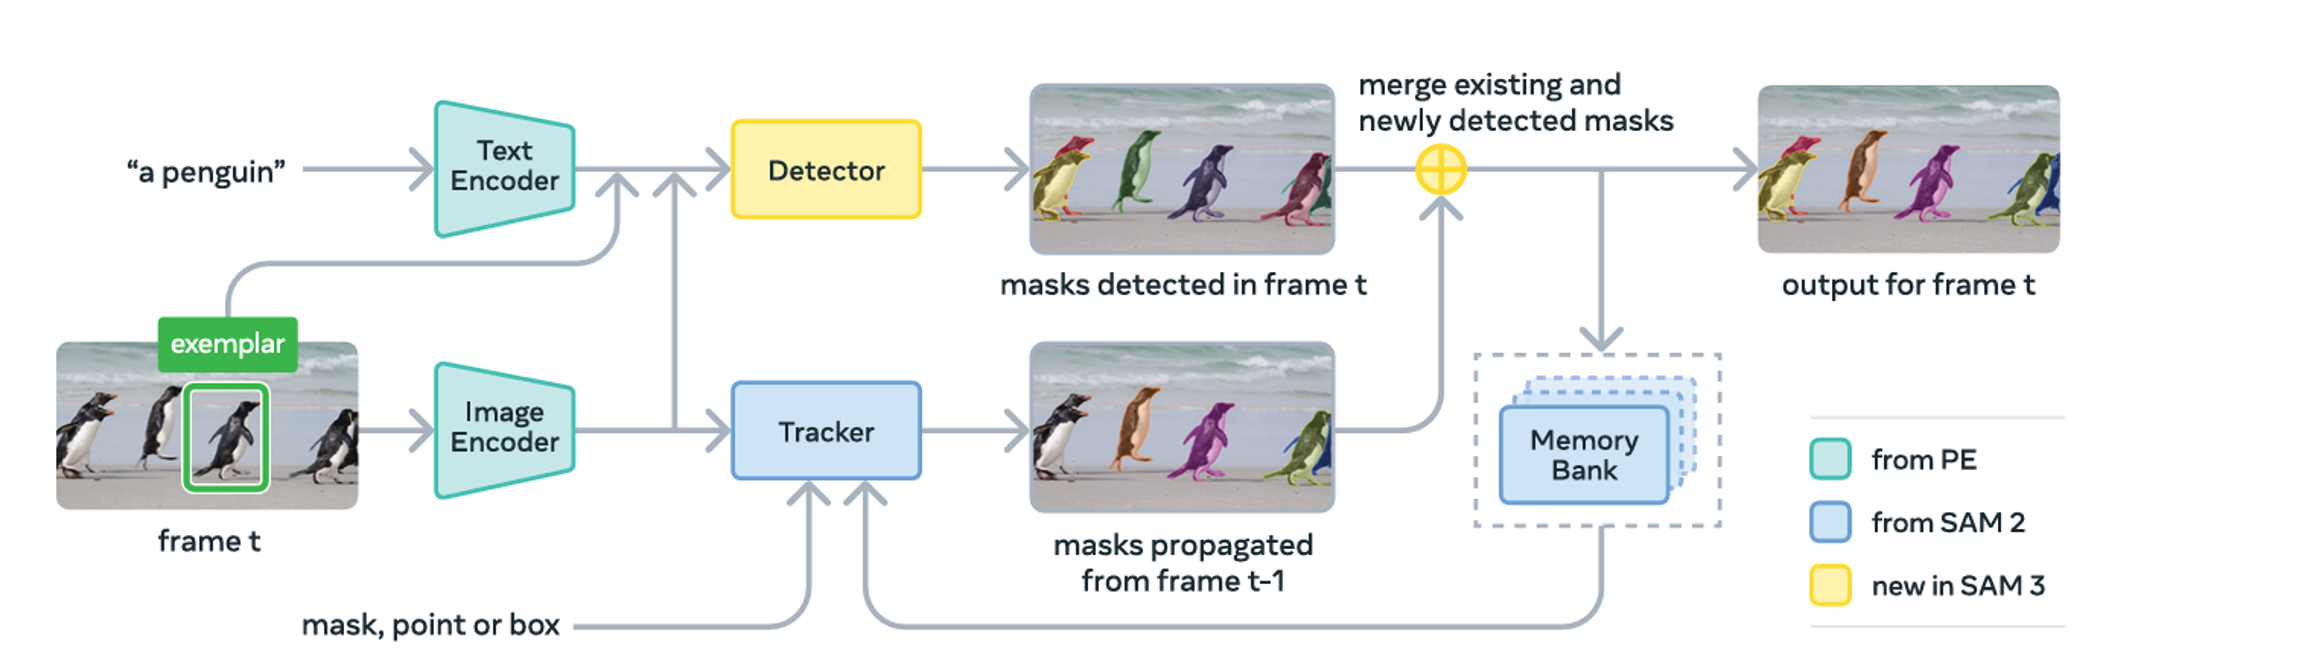
\includegraphics[width=0.7\textwidth,keepaspectratio]{lc-figures/sam3.png}
    \caption{\songti SAM3 方法示例}
    \label{fig:sam3}
\end{figure*}


这一设计能够缓解语义识别和空间定位之间的相互干扰。例如，对于外观相近但属性不同的对象，模型不仅需要找到候选区域，还需要判断该候选对象是否真正符合文本描述。

因此，SAM 3 的检测模块实际上承担了语义匹配、目标定位和实例分割等多个相互关联的功能。

\noindent\textbf{基于记忆机制的视频分割。}

除静态图像分割之外，SAM 3 还支持视频中的对象跟踪与分割。

对于连续视频，若每一帧都独立执行目标检测和分割，不仅会增加计算成本，而且可能由于遮挡、运动模糊或目标外观变化，使同一对象在不同帧之间产生不一致的分割结果。

为解决这一问题，SAM 3 引入基于记忆的视频跟踪模块，其设计延续了 SAM 2 的视频分割机制。

在处理视频时，模型可以将此前帧中的目标特征、分割结果及相关状态存入 Memory Bank，并利用这些历史信息指导当前帧的目标分割。

对于当前帧，检测器负责发现符合输入语义概念的新目标，跟踪器则根据历史记忆传播已存在目标的分割信息。随后，系统对新检测结果与已有跟踪结果进行融合，输出当前帧中符合条件的目标 Mask。

这一机制能够减少视频中重复进行人工提示的需求，并提高同一对象跨帧分割的连续性。

\noindent\textbf{数据构建与实验表现。}

为了支持开放词汇概念分割，SAM 3 构建了大规模视觉概念数据体系，涉及约 400 万个不同的概念标签，并包含用于区分相近概念的困难负样本。

这些数据不仅帮助模型学习常见物体类别，还能够增强其对对象属性、细粒度语义和复杂场景的识别能力。

原论文同时构建了 Segment Anything with Concepts（SA-Co）评测基准，用于评价模型在图像和视频概念分割中的表现。

作者报告，SAM 3 在其提出的图像和视频概念分割评测任务中，相比已有系统取得了显著提升，并进一步保留了前代 SAM 系列模型的视觉交互式分割能力。

这表明统一模型能够同时结合文本语义理解、图像目标检测以及视频时序跟踪，实现较为通用的视觉对象分割。

\noindent\textbf{方法优势与医学应用局限。}

SAM 3 的主要优势是减少对人工空间定位提示的依赖。用户不必事先知道每个目标的位置，只需输入能够描述目标的语义概念，模型即可尝试识别和分割图像中匹配的所有对象。

相比 MedSAM 主要依赖边界框的交互方式，SAM 3 在批量目标发现与语义驱动分割方面具有明显优势。

然而，SAM 3 的主要研究目标是通用视觉场景中的开放词汇对象识别与分割，其训练数据和核心评测任务并非专门围绕医学图像中的复杂病灶构建。

与自然图像相比，医学图像中的病灶可能具有模糊边界、弱对比度、细粒度形态变化等特点。此外，一些医学术语需要依赖特定的解剖位置和专业影像特征才能正确理解，不能简单等同于自然图像中的物体名称。

因此，模型能够理解一般语义概念，并不必然意味着它能够准确定位和分割复杂医学病灶。

在本项目的前期探索中，我们使用 SAM 3.1 对乳腺超声图像进行了提示分割测试。实验发现，对于部分乳腺病灶，使用医学文本提示时模型可能产生空预测或错误区域；而通过准确的位置框进行提示后，模型通常能够获得更合理的分割结果。

这一现象说明，在所测试的医学场景中，模型的边界分割能力与文本条件下的目标定位能力可能存在差异。对于以自动预标注为目标的应用，若仍需要人工提供目标位置才能获得可靠结果，则难以充分发挥文本驱动自动标注的优势。


\subsubsection{BiomedParse：医学文本驱动的联合解析}

BiomedParse 是 Zhao 等人在 Nature Methods 2025 上提出的生物医学图像基础模型\cite{biomedparse2025}。该研究将医学图像中的分割、检测和识别纳入统一框架，重点解决传统医学分割方法依赖人工位置提示，以及不同视觉任务之间缺乏协同学习的问题。

\noindent\textbf{研究背景与核心思想。}

医学图像分析通常包含三个相互关联的任务：分割（Segmentation）、检测（Detection）和识别（Recognition）。

其中，分割主要关注对象的像素级区域；检测关注对象在图像中的位置；识别则关注对象的类别及语义属性。

传统方法通常将上述任务分别处理。例如，分割模型可能要求用户提前提供目标的边界框，再根据该位置提示生成 Mask；目标检测模型负责输出候选位置，而识别模型则根据视觉特征判断对象类别。

虽然这些方法分别取得了一定进展，但将任务完全分离会造成信息利用不足。特别是在医学场景中，目标的位置、形状和语义类别通常具有密切联系。

例如，脑部肿瘤不仅具有特定的视觉纹理，还与脑组织的解剖结构、影像模态以及病变形态有关。如果模型能够同时学习这些信息，就有可能在无需人工指定位置的情况下，根据医学术语直接定位并分割目标。

基于这一思想，BiomedParse 提出统一的生物医学图像解析框架，通过联合学习分割、检测和识别任务，使模型同时获得医学视觉特征和医学语义表示。

\noindent\textbf{BiomedParseData 数据体系。}

训练医学文本驱动的分割模型，需要同时具有医学图像、像素级分割标签和相应的医学语义描述。

然而，现有公开医学数据集通常面向单一任务设计。部分数据集只提供器官或病灶分割 Mask，部分数据集提供诊断类别，而不同数据集对同一医学对象的命名方式也可能存在差异。

为解决这一问题，作者整合了 45 套生物医学图像分割数据集，利用原始数据集中已有的标签和描述信息，构建统一的医学图像解析数据体系 BiomedParseData。

该数据集包含约 340 万组不同的图像、Mask 与语义标签三元组。进一步通过扩展同义描述和专业表达，作者构建了约 680 万组图像、Mask 与文本描述三元组，覆盖九种医学影像模态。

在语义组织方面，作者构建了具有层级结构的医学对象体系。其最高层包含器官、异常结构和组织病理学对象三种主要类别；中间层包含 15 种元对象类型；细粒度层包含 82 种具体的生物医学对象类型。

为了统一不同数据集中的描述方式，作者在数据整理阶段利用 GPT-4 辅助进行术语规范化和同义描述生成，并结合医学知识体系对语义类别进行整理。

例如，作者将文本提示组织为对象类型、解剖位置和成像模态的组合形式，使模型能够同时获得需要识别的医学目标以及其对应的影像场景信息。

这种数据构建方式使得原本相互独立的医学分割数据集能够用于统一的图像--文本联合学习，从而为跨模态医学对象解析提供较为丰富的监督信息。

\noindent\textbf{模型结构与多任务联合学习。}

BiomedParse 采用基于 SEEM 的模块化架构，主要由图像编码器、文本编码器、Mask 解码器和元对象分类器构成。

其中，图像编码器负责提取医学图像中的视觉特征；文本编码器负责将输入的医学描述转换为语义特征；Mask 解码器根据视觉与文本条件输出对应目标的像素级分割概率；元对象分类器则通过预测较高层级的医学对象类别，增强模型对医学语义信息的学习。

在初始化方面，作者分别采用 Focal 网络和 PubMedBERT 的预训练表示初始化视觉编码器和文本编码器，使模型能够同时利用视觉特征提取能力与生物医学语言理解能力。

对于输入医学图像 $I$ 和文本提示 $T$，
BiomedParse 的预测过程可表示为
$P=M_{\theta}(I,T)$，
其中 $M_{\theta}$ 表示模型，$P$ 表示分割概率图。

其中，$M_{\theta}$ 表示模型，$P$ 表示与原始图像对应的分割概率图，每个像素的取值位于 $[0,1]$ 之间。

经过适当阈值处理后，可以将概率图转换为二值 Mask，用于标识文本提示指定的医学目标区域。

与基于边界框的医学分割方法不同，BiomedParse 将目标语义作为主要条件输入。模型需要同时完成目标类别理解、图像区域定位和像素级分割，而不是仅仅对已知位置中的目标绘制边界。

这种设计使得模型能够利用不同医学对象的典型形态与语义特征，对形状不规则的病灶和组织进行解析。

\noindent\textbf{文本驱动的医学图像分割流程。}

在推理阶段，BiomedParse 接收一张医学图像和一条医学文本描述，并直接生成与该描述对应的分割 Mask。

例如，对于乳腺超声图像，可以使用 tumor in breast ultrasound 作为提示；对于脑部 MRI 图像，可以使用与脑胶质瘤相关的医学描述；对于皮肤镜图像，则可以使用与皮肤病灶相关的文本提示。

模型首先通过图像编码器提取组织和病变特征，再通过文本编码器理解目标的医学语义，随后融合两类信息并生成对应的分割区域。

这一过程不需要人工提前提供目标的 Bounding Box，也不要求用户在图像中逐个点击病灶。


\begin{figure*}[!t]
    \centering
    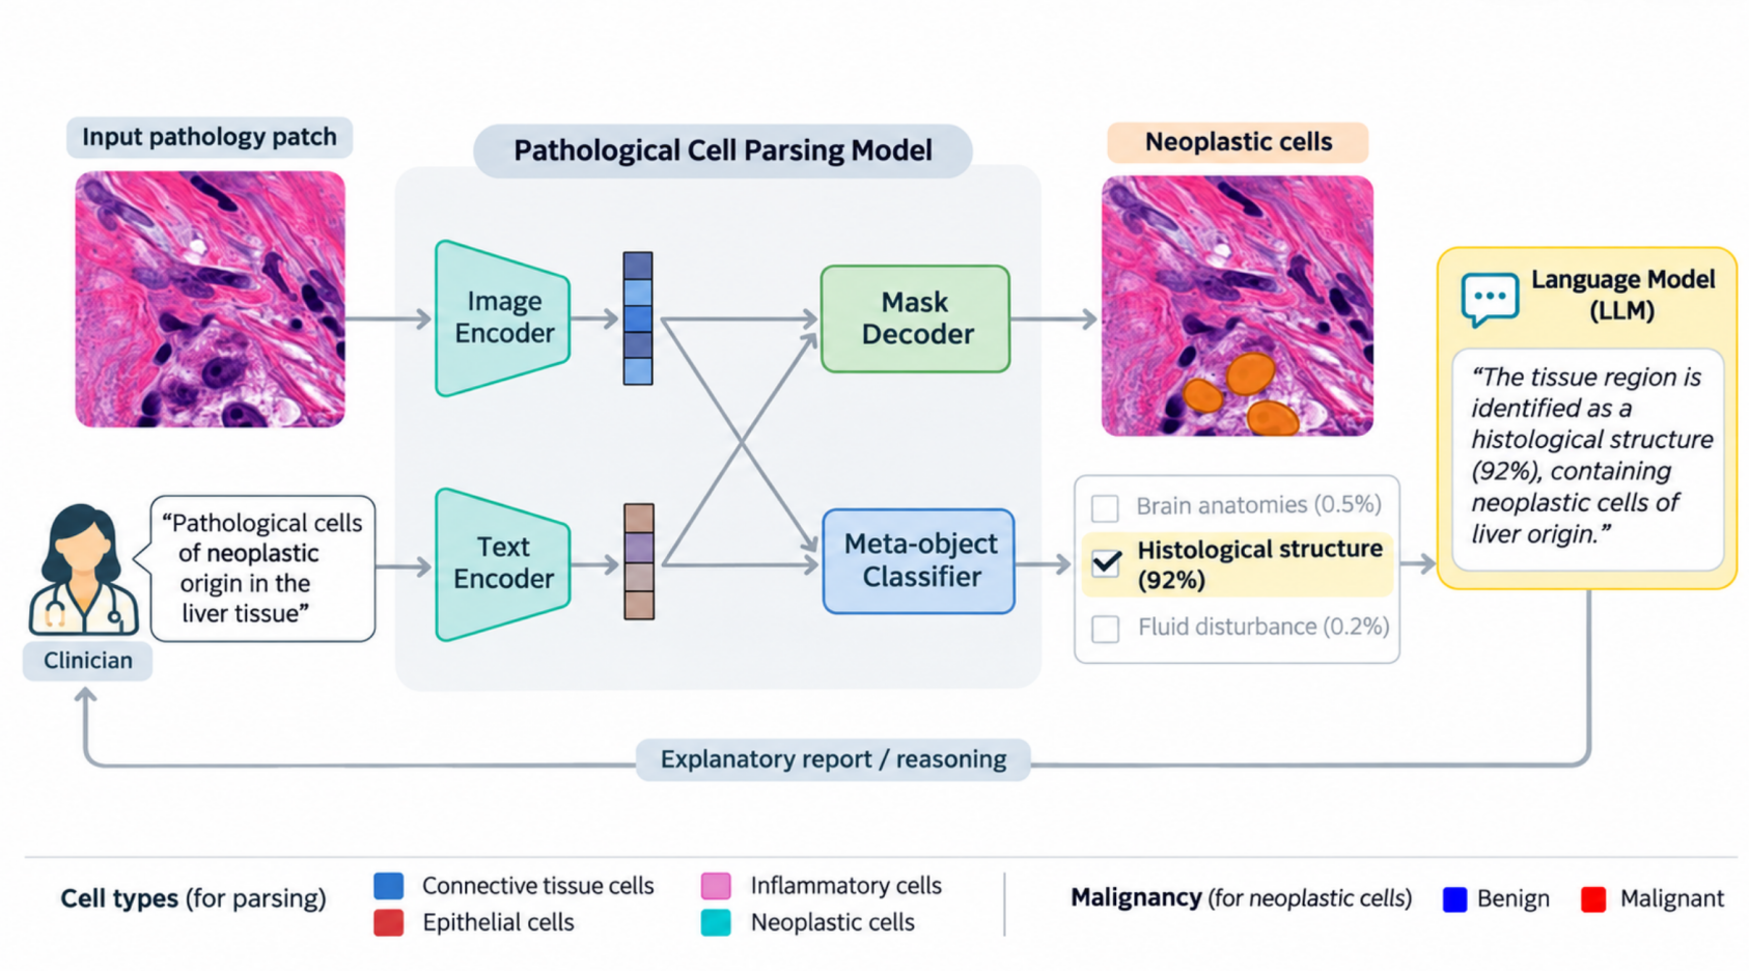
\includegraphics[width=0.7\textwidth,keepaspectratio]{lc-figures/biomedparse.png}
    \caption{\songti BiomedParse 方法示例}
    \label{fig:biomedparse}
\end{figure*}


此外，BiomedParse 还研究了无效文本提示的识别问题。当文本描述的目标并不存在于当前图像中时，模型可能由于局部像素的偶然高响应而产生错误分割。

为此，原论文设计了基于预测概率分布的统计检验方法，利用 Kolmogorov--Smirnov（K-S）检验判断图像与文本提示是否具有合理的匹配关系。

通过对无效提示进行识别和筛除，模型能够减少对不存在目标的错误预测，并进一步支持对图像中多个候选医学对象进行自动识别。

\noindent\textbf{原论文实验结果与方法优势。}

BiomedParse 的原论文在九种医学影像模态上开展了大规模评价，其中分割测试涉及 102855 组图像、Mask 与标签样本。

作者将 BiomedParse 与 SAM、MedSAM 等方法进行比较。对于需要位置框的模型，实验分别考虑由真实标注生成的理想边界框，以及由目标检测模型预测得到的边界框。

结果表明，BiomedParse 在原论文设置的多种医学分割任务中取得了具有竞争力的结果，并在部分形状不规则的医学对象上表现出更加明显的优势。

与传统基于边界框的方法相比，BiomedParse 的一个重要特点是能够直接根据语义描述指定目标。因此，当一幅图像包含多个需要分割的对象时，模型不必要求用户逐个提供位置框。

这一特点对于病理细胞、复杂病灶以及大规模医学影像预标注具有实际价值，可以减少标注人员在目标定位阶段的重复操作。

同时，模型通过医学领域数据进行联合学习，相比仅面向自然图像的通用分割方法，更加重视医学术语、医学影像模态以及目标结构之间的关联。

\noindent\textbf{方法局限与适用范围。}

尽管 BiomedParse 具有较强的医学文本驱动分割能力，但其表现仍然受到训练数据覆盖范围、目标类别和文本提示质量等因素影响。

首先，模型对医学术语的理解建立在其已有的医学语义体系和训练数据基础上。对于训练数据中较少出现的病灶类型，或者描述过于模糊的目标，模型仍可能产生定位偏差或分割错误。

其次，医学图像中可能同时存在多个视觉相似的组织结构。仅依赖文本描述并不总能完全消除目标歧义，尤其是在病灶边界模糊、异常区域较小或图像质量不佳的情况下。

再次，BiomedParse 的自动分割结果仍属于模型预测，不能直接视为经过医学专家确认的高质量标注。因此，在实际数据标注流程中，仍然需要通过人工审核及时发现错误区域并修正边界。

从应用角度来看，BiomedParse 更适合作为医学图像自动预标注模块，而不是完全替代人工审核过程。

\noindent\textbf{本项目的方法选型依据。}

综合以上代表性方法，可以发现不同模型在目标指定方式和应用条件上存在明显区别。

UniverSeg 通过少量已标注图像定义分割任务，适合已经积累一定标注样本的新任务适配；MedSAM 依赖边界框等空间提示，适合交互式精细分割；SAM 3 利用通用文本概念完成检测、分割与视频跟踪，减少了人工位置提示，但对专业医学场景的适配效果需要结合具体数据进行验证。

相比之下，BiomedParse 同时具有医学领域针对性和文本驱动目标指定能力，能够在不预先提供人工位置框的情况下，根据医学语义描述生成像素级分割结果。

本项目的研究目标并非开发新的医学图像分割基础模型，而是在开源标注系统上实现自动预标注与人工协同修正，并采用真实医学影像验证系统的可用性。

考虑到需要覆盖乳腺超声、脑部 MRI 和皮肤镜等不同二维医学影像，同时尽可能减少初始人工定位操作，本项目最终选择 BiomedParse v1 作为医学图像自动分割模块。

根据官方开源项目的版本说明，BiomedParse v1 主要面向二维医学影像，而后续版本进一步增强了三维医学影像处理能力。因此，针对本项目采用的二维医学图像数据，使用 v1 预训练模型符合项目实际需求。

在系统实现上，本项目采用 BiomedParse v1 生成分割预测结果，再将其转换为 Label Studio 支持的像素级 Mask 格式，使标注人员能够对预测区域进行查看、修改与保存。

通过这种方式，将医学文本驱动自动分割与开源标注平台的人工审核功能相结合，形成从原始医学图像到可编辑标注结果的完整流程。



















\subsection{实验结果与分析}

为评估 BiomedParse v1 在不同医学影像模态下的自动分割能力，本项目分别在 BUSI、LGG 和 ISIC 2018 三套数据集上开展实验。三套数据集分别包含乳腺超声、脑部磁共振和皮肤镜图像，在成像方式、组织结构、病灶形态及图像质量等方面存在明显差异，能够为医学图像智能标注方法提供多样化的测试场景。

实验采用 BiomedParse v1 官方发布的预训练模型，不对模型参数进行额外微调。对于不同数据集，根据其医学影像类型和目标病灶选择相应的医学文本提示，由模型生成像素级分割结果，并与数据集提供的人工标注进行比较。


\noindent\textbf{整体定量实验结果。}

表~\ref{tab:biomedparse_results} 给出了 BiomedParse v1 在三套医学影像数据集上的自动分割结果。其中，BUSI 数据集的平均 Dice 和 IoU 分别为 0.7965 和 0.7007；LGG 数据集分别为 0.9173 和 0.8512；ISIC 2018 数据集分别为 0.8735 和 0.7925。

\begin{table}[htbp]
\centering
\caption{BiomedParse v1 在三个医学影像数据集上的分割结果}
\label{tab:biomedparse_results}
\vspace{1.5mm}
\resizebox{\columnwidth}{!}{%
\begin{tabular}{l l c c}
\toprule
数据集 & 影像模态 & Dice $\uparrow$ & IoU $\uparrow$ \\
\midrule
BUSI & 乳腺超声 & 0.7965 & 0.7007 \\
LGG & 脑部 MRI & 0.9173 & 0.8512 \\
ISIC 2018 & 皮肤镜 & 0.8735 & 0.7925 \\
\bottomrule
\end{tabular}%
}
\end{table}

从总体结果来看，BiomedParse v1 在三种成像模态上均获得了非零且具有一定重合程度的病灶分割结果。其中，LGG 和 ISIC 2018 数据集的平均 Dice 均超过 0.87，BUSI 数据集的平均 Dice 接近 0.80。这说明在当前选取的测试样本中，模型能够利用医学文本提示生成与人工标注区域具有较高重合度的预测 Mask。

从评价指标之间的关系来看，三个数据集上的 Dice 与 IoU 呈现一致的性能排序，即 LGG 最优，ISIC 2018 次之，BUSI 相对较低。这一现象说明，两项指标对当前实验中不同数据集分割质量的整体评价具有一致性。

Dice 和 IoU 均以预测区域与真实区域的空间重合程度为基础，但两者对重合关系的度量方式不同。IoU 以交集和并集的比值衡量分割质量，而 Dice 对交集赋予双倍权重。因此，在相同的预测结果下，IoU 通常低于 Dice。

\noindent\textbf{乳腺超声图像上的分割表现。}

在 BUSI 数据集上，BiomedParse v1 取得了 0.7965 的平均 Dice 和 0.7007 的平均 IoU。与其他两套数据集相比，BUSI 上的指标相对较低，说明模型在当前测试的乳腺超声图像中仍然存在一定程度的预测区域偏差。

这一现象可能与乳腺超声的成像特点有关。超声成像主要利用组织之间的声学特性差异生成图像，其结果容易受到散斑噪声、声衰减、组织回声差异及成像伪影的影响。相比部分边界较清晰的目标，乳腺肿块可能与周围正常组织具有相近的灰度分布，导致病灶与背景之间缺乏明显的视觉分界。


\noindent\textbf{脑部 MRI 图像上的分割表现。}

在 LGG 数据集上，BiomedParse v1 的平均 Dice 达到 0.9173，平均 IoU 达到 0.8512，是本次实验中表现最好的数据集。

与 BUSI 相比，LGG 的平均 Dice 高出 0.1208，平均 IoU 高出 0.1505；与 ISIC 2018 相比，其平均 Dice 高出 0.0438，平均 IoU 高出 0.0587。这表明在本项目选取的脑部 MRI 测试样本中，模型预测区域与人工标注之间具有更高的平均重合程度。

LGG 数据集使用的 FLAIR 序列能够抑制脑脊液信号，使部分脑组织异常区域在图像中表现为相对明显的信号变化。对于一些与正常组织形成较强信号差异的异常区域，模型可能更容易提取与分割目标相关的视觉特征。

与此同时，BiomedParse v1 在预训练阶段接触了包含 MRI 在内的多种医学影像数据，其学习到的医学视觉表示可能有助于识别脑部 MRI 中的异常组织区域。

对于本项目的智能标注系统而言，LGG 实验表明，在当前选取的 MRI 图像中，BiomedParse v1 能够生成与人工标注较为接近的预测结果，为后续的人工审核和精细修正提供较好的初始 Mask。

\noindent\textbf{皮肤镜图像上的分割表现。}

在 ISIC 2018 数据集上，BiomedParse v1 的平均 Dice 为 0.8735，平均 IoU 为 0.7925，整体表现介于 LGG 和 BUSI 之间。

与 BUSI 相比，ISIC 2018 的平均 Dice 高出 0.0770，平均 IoU 高出 0.0918，说明在当前测试样本中，模型对皮肤镜病灶区域的预测与人工标注具有更高的空间重合程度。

与超声和 MRI 不同，皮肤镜图像通常具有丰富的颜色和纹理信息。部分皮肤病灶与周围正常皮肤之间存在明显的色素差异，可以为模型提供较为直观的目标定位线索。

但皮肤镜图像同样存在多种影响分割准确性的因素。例如，不同病灶的颜色、纹理、形状和尺寸可能存在较大差异；部分病灶边缘颜色逐渐过渡，与周围正常皮肤缺乏明确分界；图像中的毛发、反光、气泡和局部光照变化也可能干扰模型对病灶边界的判断。

对于自动分割模型而言，即使能够根据整体颜色和纹理信息识别病灶的大致位置，也不一定能够完全恢复其不规则边界。特别是当病灶边缘存在颜色渐变、局部遮挡或细小突起时，预测 Mask 与人工标注之间仍可能出现差异。

因此，ISIC 2018 上的实验结果说明 BiomedParse v1 能够对彩色皮肤镜图像进行有效的病灶预标注，但对于边界复杂或存在明显干扰因素的图像，仍有必要由人工进一步确认分割轮廓。

综合 BUSI、LGG 和 ISIC 2018 的实验结果可以看出，同一预训练模型在不同医学影像上的分割表现存在差异。影响这种差异的因素可能包括影像模态、目标形态、图像质量、训练数据覆盖程度以及文本提示与目标之间的语义匹配程度。

\noindent\textbf{自动分割结果的可视化分析。}

除 Dice 和 IoU 等定量指标外，本项目还通过可视化方式展示模型生成的分割结果，以更加直观地观察自动预测区域与人工标注之间的对应关系。

图~\ref{fig:biomedparse_visualization} 展示了 BiomedParse v1 在医学影像上的分割结果示例。通过将原始医学图像、数据集提供的人工分割 Mask 与模型预测结果进行对照，可以观察不同成像条件下模型对目标区域的定位和边界恢复情况。

\begin{figure}[!htbp]
    \centering
    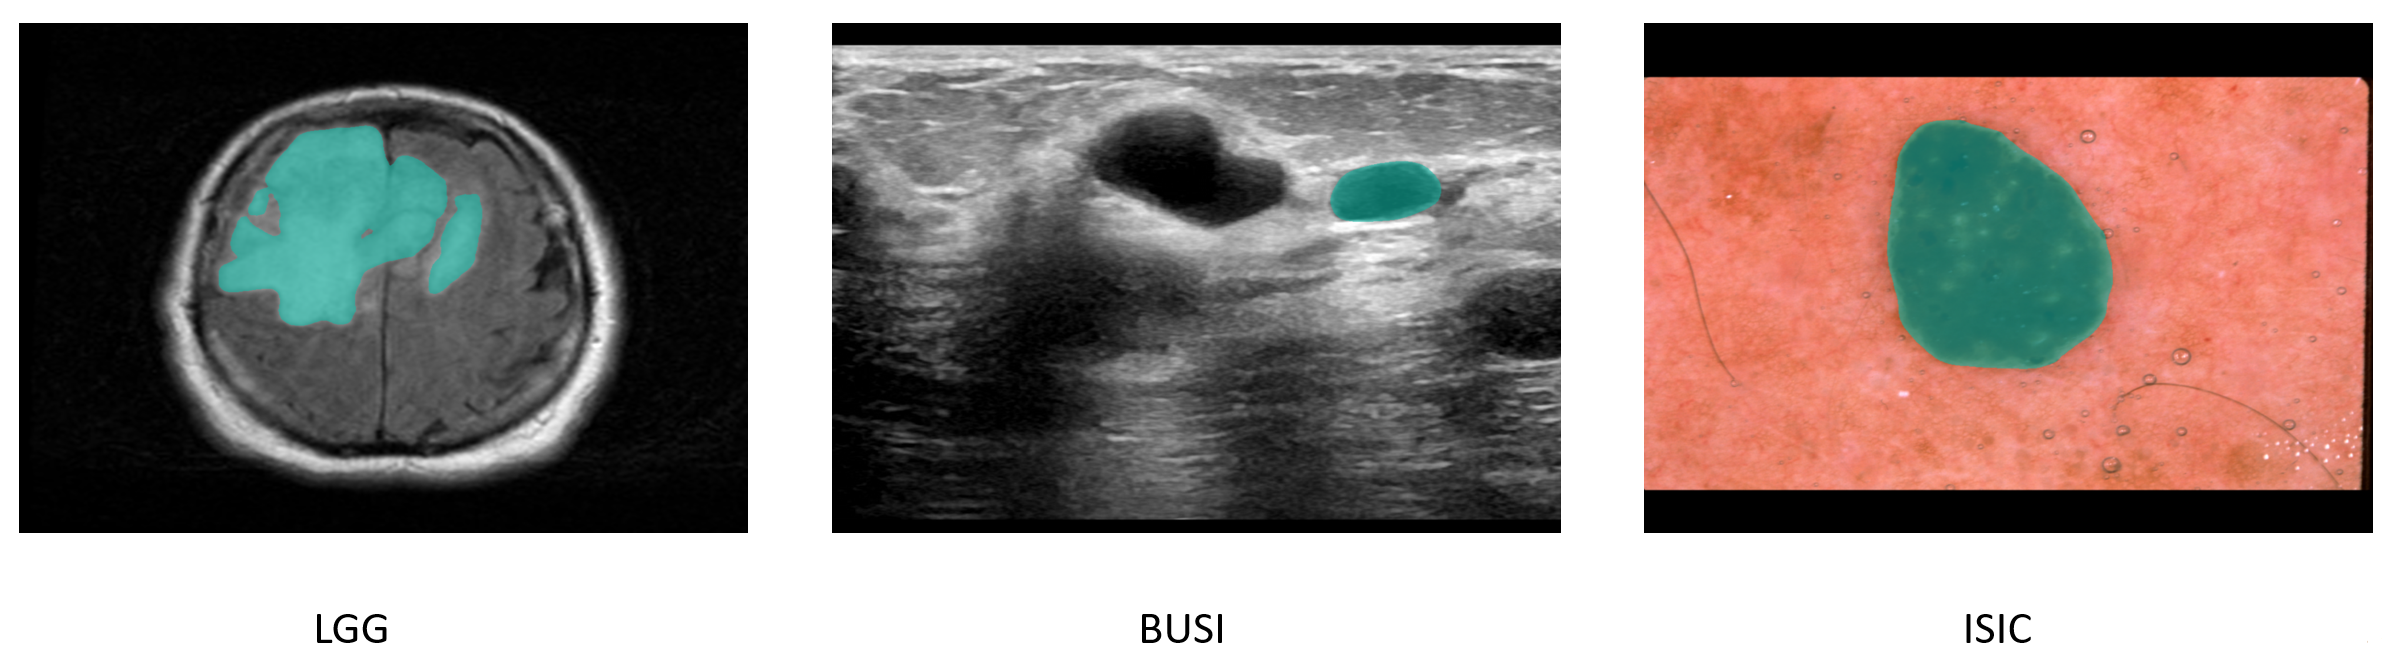
\includegraphics[width=\linewidth,keepaspectratio]{lc-figures/result.png}
    \caption{\songti BiomedParse v1 医学图像自动分割结果可视化}
    \label{fig:biomedparse_visualization}
\end{figure}

与单纯报告平均指标相比，结果可视化能够提供更加直观的空间信息。Dice 和 IoU 可以量化整体区域的重合程度，但无法完整反映分割误差在图像中的具体位置。例如，两张图像可能具有相近的 Dice 值，但其错误区域可能分别集中于病灶边缘和病灶内部，因而对后续人工修正产生不同影响。

在医学图像自动标注任务中，预测结果通常不要求完全替代人工标注，而是为人工审核提供初始参考。因此，除了整体分割精度之外，预测 Mask 是否覆盖主要目标区域、是否包含明显的无关区域，以及错误区域是否容易通过交互工具进行修正，也是评价系统实用性的重要因素。

对于边界较为准确的预测结果，标注人员可以直接确认并保存；对于存在局部偏差的结果，可以通过画笔或橡皮擦进行补充和修正；对于定位明显错误或预测区域缺失的情况，则需要重新指定或绘制标注区域。

由此可见，自动分割模型的作用不仅在于输出最终 Mask，还在于为医学图像标注人员提供可编辑的初始结果，减少从零开始绘制病灶区域的工作需求。



\noindent\textbf{本节小结。}

综合实验结果，BiomedParse v1 在本项目选取的 BUSI、LGG 和 ISIC 2018 样本上均能够生成与人工标注具有较高空间重合度的病灶分割结果，其中 LGG 的平均 Dice 和 IoU 分别达到 0.9173 和 0.8512，表现相对较好；BUSI 上的平均 Dice 和 IoU 分别为 0.7965 和 0.7007，说明乳腺超声病灶自动分割仍存在一定的改进空间。

上述结果表明，在不进行额外模型训练的条件下，利用医学文本提示驱动的预训练分割模型，可以为不同医学影像类型提供统一的自动预标注能力。

然而，考虑到医学图像的复杂性以及模型预测仍然存在误差，自动生成的 Mask 需要与人工审核机制结合使用。因此，本项目进一步将 BiomedParse v1 的分割结果接入 Label Studio 标注平台，通过可视化展示、人工交互修正和结果保存等功能，构建面向医学图像的智能辅助标注流程。






\subsection{基于 Label Studio 的人机协同标注}

前述实验验证了 BiomedParse v1 在三类医学影像上的自动分割能力，但离线分割结果并不能直接等同于实际标注系统中的可用标注数据。对于医学影像中的病灶区域，模型预测仍可能存在边界偏差、局部区域遗漏或背景误检等问题，需要通过人工审核进一步保证标注质量。

因此，本项目在完成医学图像自动分割实验的基础上，进一步将 BiomedParse v1 与 Label Studio 标注平台进行集成，实现模型预测结果的可视化展示、人工交互修正以及标注结果保存。与传统完全由人工绘制病灶轮廓的方式不同，本项目利用预训练医学分割模型生成初始 Mask，再由标注人员对预测结果进行确认和必要的局部修改，形成面向医学图像的人机协同标注流程。

\noindent\textbf{BiomedParse 自动分割结果接入}

对于每张医学图像，首先利用 BiomedParse v1 进行自动分割推理。模型根据输入的医学图像和相应的医学文本提示，输出目标病灶的像素级分割结果。

由于 BiomedParse 的预测结果以分割 Mask 形式表示，而 Label Studio 使用特定的数据结构管理图像标注区域，因此需要对模型输出进行格式转换，以满足平台对预标注数据的要求。

具体而言，本项目首先将模型输出整理为与原始图像对应的分割掩码，并根据当前医学任务设置相应的类别标签。随后，将分割区域转换为 Label Studio 支持的预测数据格式，并与平台中对应的医学图像任务建立关联。

在数据转换过程中，需要保证预测 Mask 与原始图像之间的尺寸和空间位置一致，避免因图像缩放或格式转换导致分割区域发生偏移。

对于 BUSI 数据集，系统使用 Tumor 标签表示乳腺肿块区域；对于 LGG 和 ISIC 2018 数据集，则根据相应的医学分割任务配置目标类别。

完成转换后，将模型预测结果作为 Prediction 导入 Label Studio，而不是直接作为已经完成审核的人工 Annotation。这样既能够保留模型自动生成的原始结果，也能够将预测区域作为后续人工审核的初始参考。


\noindent\textbf{医学图像自动预标注展示。}

模型预测结果成功接入平台后，标注人员可以直接打开医学图像任务，查看 BiomedParse v1 自动生成的分割区域。

与仅展示原始医学图像不同，系统会在图像中叠加显示模型预测的病灶 Mask，使标注人员能够直观观察病灶的位置、范围及边界。

对于乳腺超声图像，预标注主要用于显示乳腺肿块区域；对于脑部 MRI 图像，预标注用于显示胶质瘤相关异常信号区域；对于皮肤镜图像，则用于显示皮肤病灶轮廓。

三类图像虽然具有不同的成像特点，但均能够通过统一的像素级分割标注方式展示模型预测结果。这说明 BiomedParse v1 生成的不同医学影像分割结果可以经过统一的数据转换流程接入同一标注平台，而不需要为每一种医学影像重新开发独立的标注界面。

与此同时，模型预测区域与原始医学图像能够正确对应，标注人员可以结合影像中的实际组织结构判断分割结果是否合理。

对于预测较为准确的样本，标注人员只需要检查病灶区域是否完整；对于预测存在明显偏差的样本，则需要进一步检查遗漏区域、错误包含的背景区域及局部边界。

这一实现将原本只能在离线实验中查看的模型预测结果转化为可交互的预标注数据，为后续人工质量控制提供了基础。

\noindent\textbf{原始 Mask 的人工修正与保存}

考虑到医学图像分割模型难以保证所有病灶区域均被准确识别，本项目进一步验证了模型预测 Mask 在 Label Studio 中的可编辑性。

在实际标注过程中，标注人员首先查看 BiomedParse v1 生成的预标注结果，再将其复制为可编辑的人工标注区域。随后，选择对应的目标类别，并通过平台提供的画笔和橡皮擦工具对原始 Mask 进行修改。

对于模型未能完整覆盖的真实病灶区域，可以使用画笔工具补充分割像素；对于被模型错误识别为病灶的背景区域，则可以使用橡皮擦工具删除多余像素。

与重新绘制完整病灶轮廓不同，这种操作直接在模型已有预测结果的基础上进行局部修正，能够保留预测正确的区域，使人工操作主要集中于存在误差的部分。

本项目重点验证了对原有预测区域进行修改的能力，而不仅仅是在图像上重新绘制一个独立的分割区域。

以 BUSI 乳腺超声标注任务为例，首先将 BiomedParse v1 生成的 Tumor Mask 导入标注平台，在确认预测区域正常显示后，将其转换为可编辑的人工标注。

随后，通过选择已有的 Tumor 区域，使用画笔工具在原始分割结果之外增加局部像素区域，验证系统能否在保留原始 Mask 的基础上完成修改。

实验中，原有病灶分割区域能够正常保留，新增加的标注区域也能够正确显示，说明平台支持对模型预标注结果进行交互式编辑。

完成人工修改后，进一步通过 Submit 操作提交当前 Annotation。平台显示标注保存成功，表明修改后的分割结果能够作为人工标注提交并保存。


\begin{figure}[!htbp]
    \centering
    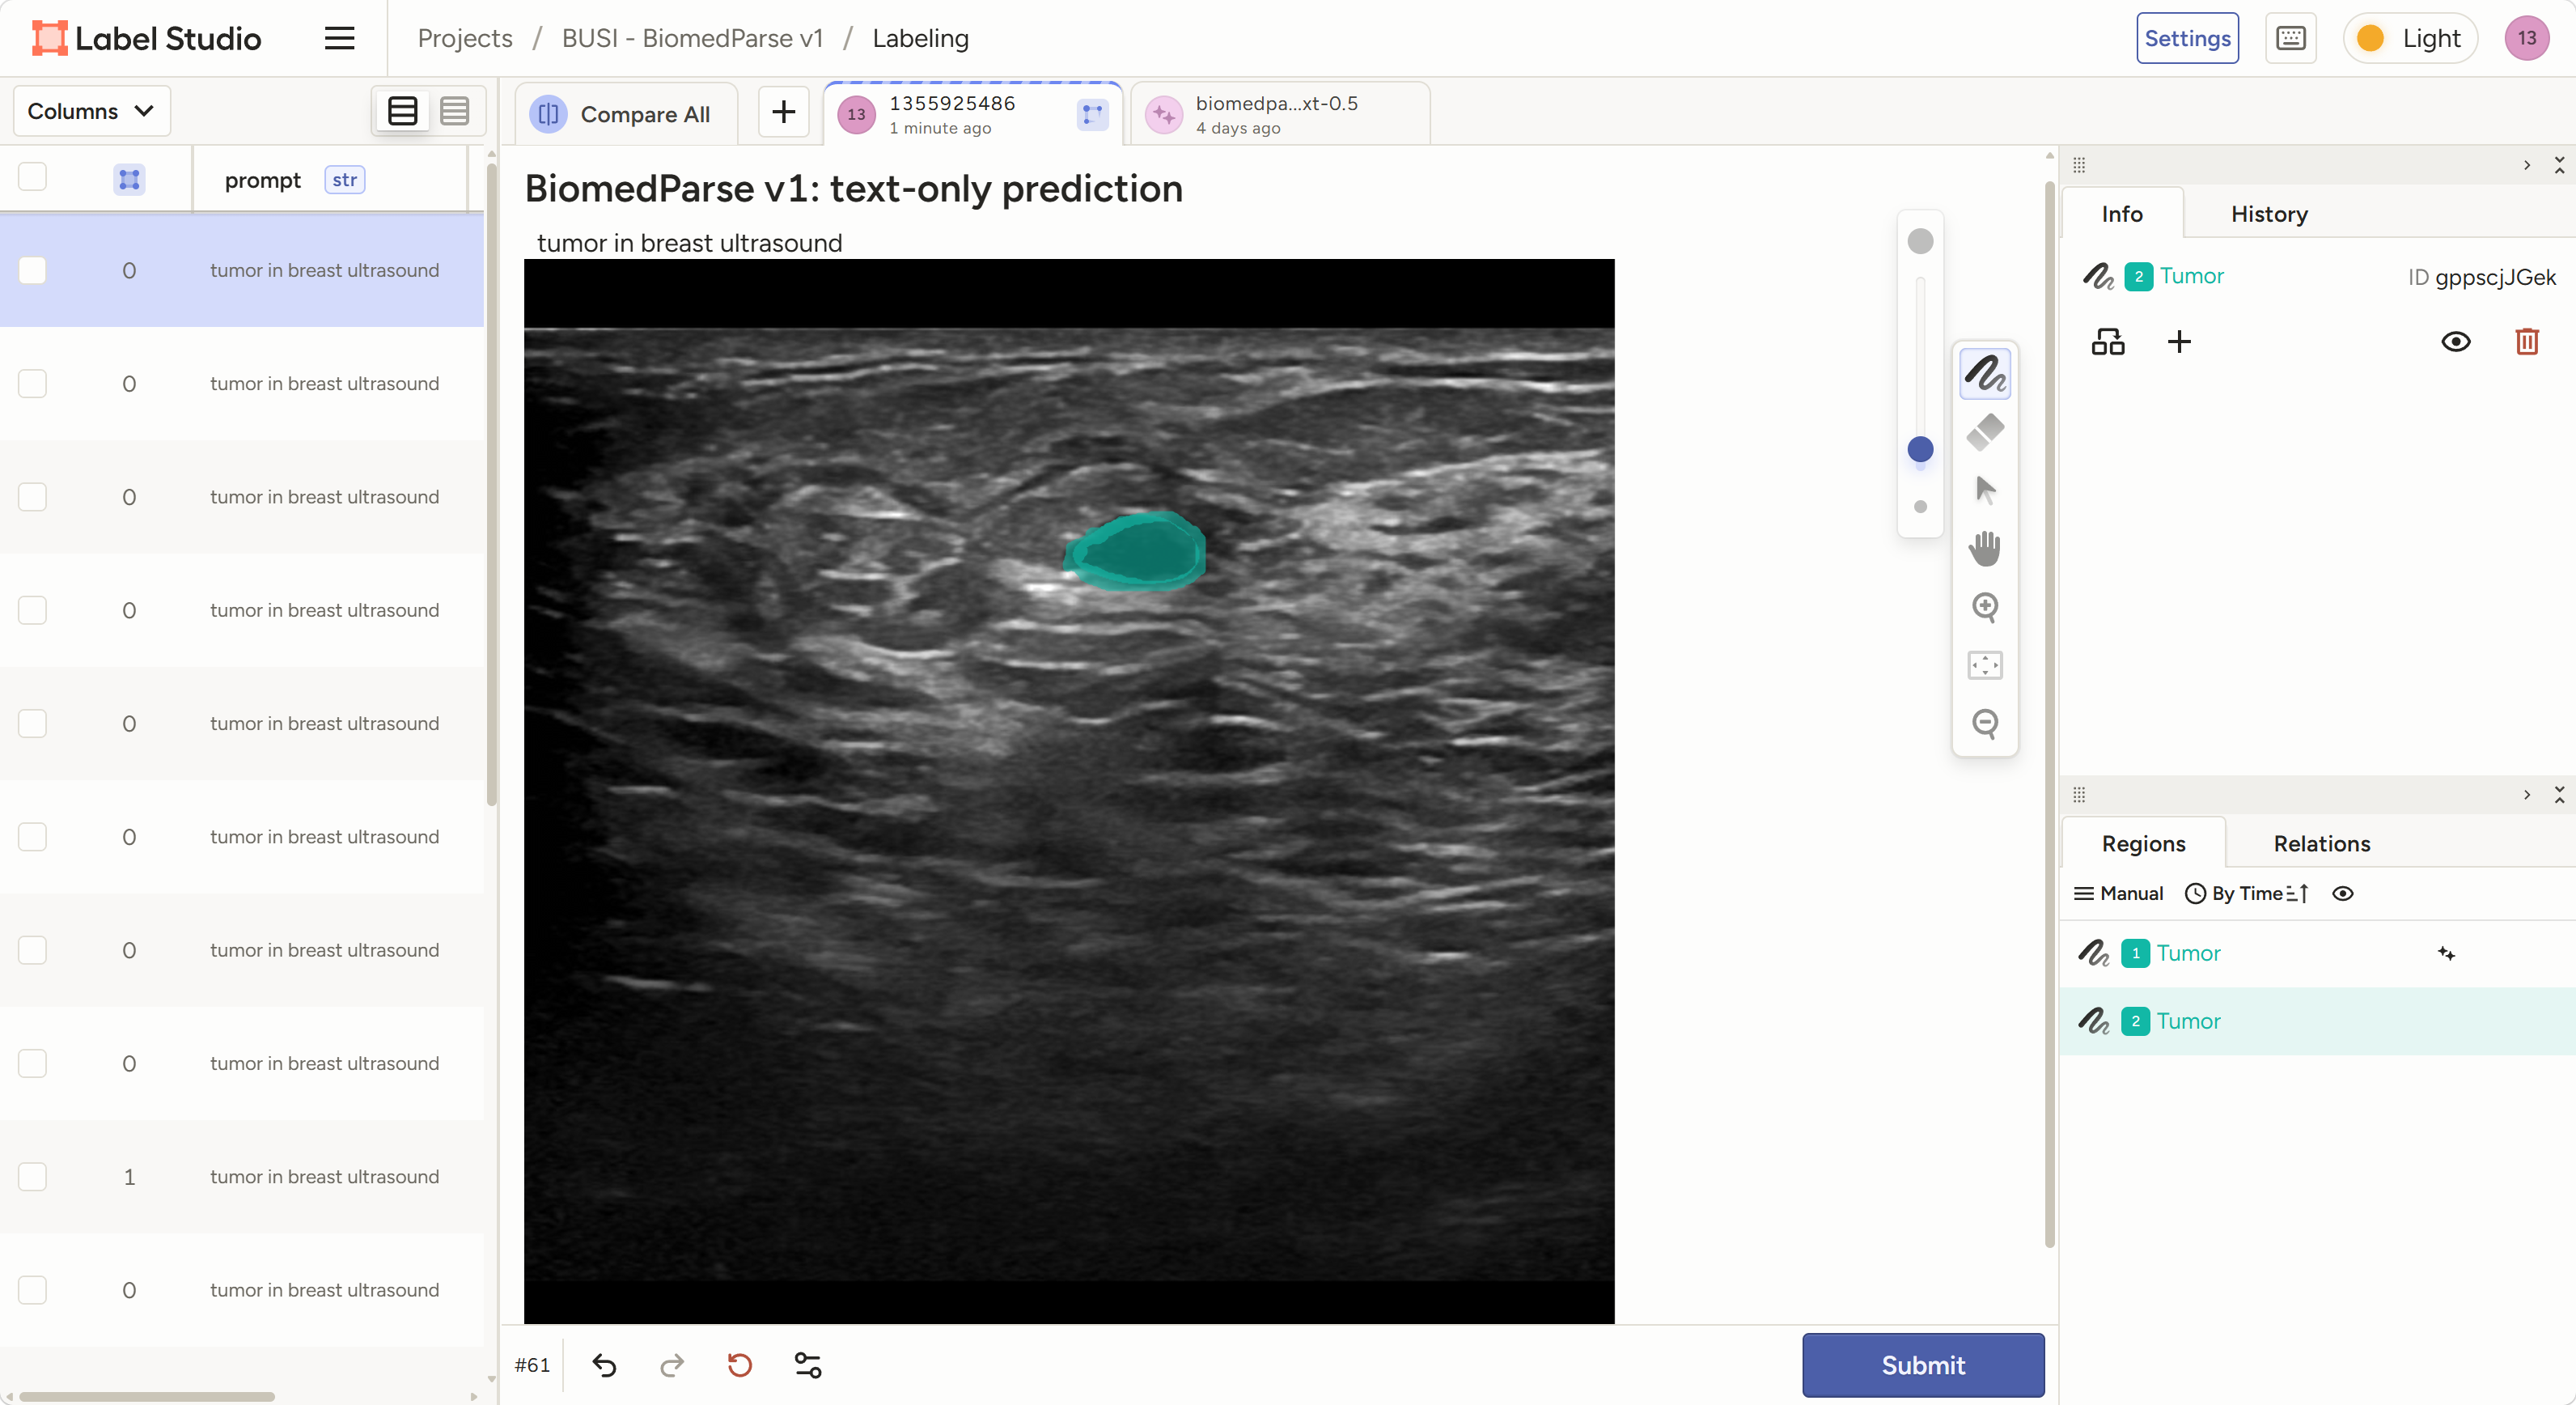
\includegraphics[width=\linewidth,keepaspectratio]{lc-figures/界面展示.png}
    \caption{\songti Label Studio 界面展示}
    \label{fig:biomedparse_visualization}
\end{figure}



上述实验验证了从模型自动预测、复制预标注、人工修改到标注提交保存的主要操作流程。


\noindent\textbf{系统功能验证与结果分析}

为检验所构建医学图像智能辅助标注流程的可用性，本项目分别从自动预标注、人工交互和结果管理三个方面进行了验证。

在自动预标注方面，BiomedParse v1 已完成 BUSI、LGG 和 ISIC 2018 三套数据集的实际推理，生成的分割结果能够与原始医学图像对应，并成功导入 Label Studio。

在人工交互方面，标注人员能够查看预测 Mask，并利用画笔及橡皮擦对已有区域进行修改。实际操作已经验证了在原始分割区域基础上增加和删除像素的功能，说明预测结果能够作为人工标注的初始状态，而非只能进行静态展示。

在结果管理方面，系统能够保存人工修改后的 Annotation，并已完成自动预测结果的导出功能检查。对于人工修改后 Mask 的完整导出及像素级一致性，还需要结合最终导出文件进行进一步核验。

综合上述验证结果，本项目已经完成了医学图像自动预标注与人工审核功能的基本集成，实现了 BiomedParse v1 与 Label Studio 之间的预测结果传递和交互式编辑。

这一实现具有两方面的实际意义。

首先，利用 BiomedParse v1 的医学文本驱动分割能力，系统可以在不要求标注人员提前绘制病灶边界框的情况下，为不同医学影像自动生成初始分割区域。

其次，借助 Label Studio 的人工编辑机制，标注人员能够对模型预测中的错误进行修正，使自动分割结果进入可审核、可修改、可保存的数据标注流程。

不过，自动预标注能否在实际工作中提高标注效率，仍然取决于模型预测质量和人工修正成本。当模型预测较为准确时，标注人员可以主要进行确认和少量局部修正；当模型预测存在较大偏差时，人工修改工作量可能增加。

因此，本项目将 BiomedParse v1 定位为医学图像智能辅助标注模块，而不是完全替代人工审核的自动标注工具。

总体而言，本项目完成了从医学影像输入、模型自动分割、预测结果接入，到人工修正与标注保存的主要工作流程，验证了医学文本驱动分割模型在开源标注平台中的实际应用可行性。





\renewcommand{\refname}{\centering 参~考~文~献}

\begin{thebibliography}{99}
\zihao{5-}
\addtolength{\itemsep}{-1em}
\vspace{1.5mm}

\bibitem{busi2020}
Al-Dhabyani W, Gomaa M, Khaled H, Fahmy A.
Dataset of breast ultrasound images[J].
Data in Brief, 2020, 28: 104863.
DOI: 10.1016/j.dib.2019.104863.

\bibitem{lgg2019}
Buda M, Saha A, Mazurowski M A.
Association of genomic subtypes of lower-grade gliomas
with shape features automatically extracted by a
deep learning algorithm[J].
Computers in Biology and Medicine, 2019, 109: 218--225.
DOI: 10.1016/j.compbiomed.2019.05.002.

\bibitem{isic2018}
Codella N C F, Rotemberg V, Tschandl P, et al.
Skin lesion analysis toward melanoma detection 2018:
A challenge hosted by the International Skin Imaging
Collaboration (ISIC)[EB/OL].
arXiv:1902.03368, 2019.


\bibitem{universeg2023}
Butoi V I, Gonzalez Ortiz J J, Ma T, et al.
UniverSeg: Universal medical image segmentation[C]//
Proceedings of the IEEE/CVF International Conference
on Computer Vision.
2023: 21438--21451.

\bibitem{medsam2024}
Ma J, He Y, Li F, et al.
Segment anything in medical images[J].
Nature Communications, 2024, 15: 654.

\bibitem{sam32026}
Carion N, Gustafson L, Hu Y T, et al.
SAM 3: Segment Anything with Concepts[C]//
Proceedings of the International Conference
on Learning Representations.
2026.

\bibitem{biomedparse2025}
Zhao T, Gu Y, Yang J, et al.
A foundation model for joint segmentation, detection
and recognition of biomedical objects across nine
modalities[J].
Nature Methods, 2025, 22(1): 166--176.



\end{thebibliography}




 
\end{document}

